%%%%%%%%%%%%%%%%%%%%%%%%%%%%%%%%%%%%%%%%%
% Short Sectioned Assignment LaTeX Template Version 1.0 (5/5/12)
% This template has been downloaded from: http://www.LaTeXTemplates.com
% Original author:  Frits Wenneker (http://www.howtotex.com)
% License: CC BY-NC-SA 3.0 (http://creativecommons.org/licenses/by-nc-sa/3.0/)
%%%%%%%%%%%%%%%%%%%%%%%%%%%%%%%%%%%%%%%%%

%----------------------------------------------------------------------------------------
%	PACKAGES AND OTHER DOCUMENT CONFIGURATIONS
%----------------------------------------------------------------------------------------

\documentclass[a4paper, 12pt]{report} % A4 paper and 11pt font size

% ---- Entrada y salida de texto -----

\usepackage[T1]{fontenc} % Use 8-bit encoding that has 256 glyphs
\usepackage[utf8]{inputenc}
\usepackage{ascii}  
\usepackage{lilyglyphs}
\usepackage{fontspec}
%\usepackage{fourier} % Use the Adobe Utopia font for the document - comment this line to return to the LaTeX default

% ---- Idioma --------

\usepackage[spanish, es-tabla]{babel} % Selecciona el español para palabras introducidas automáticamente, p.ej. "septiembre" en la fecha y especifica que se use la palabra Tabla en vez de Cuadro

% ---- Otros paquetes ----

\usepackage{amsmath,amsfonts,amsthm} % Math packages
%\usepackage{graphics,graphicx, floatrow} %para incluir imágenes y notas en las imágenes
\usepackage{graphics,graphicx, float} %para incluir imágenes y colocarlas
\usepackage{epstopdf}
\usepackage{caption} 
\usepackage[bookmarks = true, colorlinks=true, linkcolor = black, citecolor = magenta, menucolor = black, urlcolor = blue]{hyperref} 
\usepackage{url}
\usepackage{color}
\definecolor{gray97}{gray}{.97}
\definecolor{gray75}{gray}{.75}
\definecolor{gray45}{gray}{.45}

\usepackage{listings}
\lstset{
frame=tb,
language=Pascal,
breaklines=true,
showstringspaces=false,
columns=flexible,
numbers=none,
commentstyle=\color{dkgreen},
stringstyle=\color{mauve},
tabsize=3
 }

\lstset{basicstyle=\footnotesize\ttfamily,breaklines=true}
\usepackage{parskip}

% Para hacer tablas comlejas
%\usepackage{multirow}
%\usepackage{threeparttable}

%\usepackage{sectsty} % Allows customizing section commands
%\allsectionsfont{\centering \normalfont\scshape} % Make all sections centered, the default font and small caps

\usepackage{fancyhdr} % Custom headers and footers
\pagestyle{fancyplain} % Makes all pages in the document conform to the custom headers and footers
\fancyhead{} % No page header - if you want one, create it in the same way as the footers below
\fancyfoot[L]{} % Empty left footer
\fancyfoot[C]{} % Empty center footer
\fancyfoot[R]{\thepage} % Page numbering for right footer
\renewcommand{\headrulewidth}{0pt} % Remove header underlines
\renewcommand{\footrulewidth}{0pt} % Remove footer underlines
\setlength{\headheight}{13.6pt} % Customize the height of the header

\numberwithin{equation}{section} % Number equations within sections (i.e. 1.1, 1.2, 2.1, 2.2 instead of 1, 2, 3, 4)
\numberwithin{figure}{section} % Number figures within sections (i.e. 1.1, 1.2, 2.1, 2.2 instead of 1, 2, 3, 4)
\numberwithin{table}{section} % Number tables within sections (i.e. 1.1, 1.2, 2.1, 2.2 instead of 1, 2, 3, 4)

\setlength\parindent{0pt} % Remov%Para conseguir que en las páginas en blanco no ponga cabecerass

\makeatletter
\def\clearpage{%
  \ifvmode
    \ifnum \@dbltopnum =\m@ne
      \ifdim \pagetotal <\topskip
        \hbox{}
      \fi
    \fi
  \fi
  \newpage
  \thispagestyle{empty}
  \write\m@ne{}
  \vbox{}
  \penalty -\@Mi
}
%\makeatotheres all indentation from paragraphs - comment this line for an assignment with lots of text

\makeatletter

\newcommand\frontmatter{%
    \cleardoublepage
  %\@mainmatterfalse
  \pagenumbering{roman}}

\newcommand\mainmatter{%
    \cleardoublepage
 % \@mainmattertrue
  \pagenumbering{arabic}}

\newcommand\backmatter{%
  \if@openright
    \cleardoublepage
  \else
    \clearpage
  \fi
 % \@mainmatterfalse
   }

\makeatother

\usepackage{titlesec}
\titleformat{\chapter}[display]   
{\normalfont\huge\bfseries}{\chaptertitlename\ \thechapter}{20pt}{\Huge}   
\titlespacing*{\chapter}{0pt}{-50pt}{40pt}

\usepackage{geometry}% http://ctan.org/pkg/geometry
\newcommand{\mygeometry}[1]{%
  \geometry{right=#1,left=\dimexpr#1\relax}% Set new geometry
}
\mygeometry{30mm}% 25mm left/right margins

\newcommand{\horrule}[1]{\rule{\linewidth}{#1}} % Create horizontal rule command with 1 argument of height
\usepackage{titlesec}
\titleformat{\chapter}[block]
  {\normalfont\Huge\bfseries}{\thechapter.}{1em}{\Huge}
\titlespacing*{\chapter}{0pt}{-19pt}{10pt}

\titleformat{\section}[block]
  {\normalfont\LARGE\bfseries}{\thesection.}{1em}{\normalfont\LARGE\bfseries}

 \titleformat{\subsection}[block]
  {\normalfont\large\bfseries}{\thesubsection.}{1em}{\normalfont\large\bfseries}

  \titleformat{\subsubsection}[block]
  {\normalfont\normalsize\bfseries}{\thesubsubsection.}{1em}{\normalfont\normalsize\bfseries}

\usepackage{xcolor}
\usepackage{colortbl}
\usepackage{musixtex}
\usepackage{enumitem}
%----------------------------------------------------------------------------------------
%	TÍTULO Y DATOS DEL ALUMNO
%----------------------------------------------------------------------------------------
\begin{document}

\begin{titlepage}
 
\newlength{\centeroffset}
\setlength{\centeroffset}{-0.5\oddsidemargin}
\addtolength{\centeroffset}{0.5\evensidemargin}
\thispagestyle{empty}

\noindent\hspace*{\centeroffset}
\begin{minipage}{\textwidth}

\centering

\includegraphics[width=0.9\textwidth]{imagenes/logo_ugr.jpg}\\[1.4cm]

\textsc{ \Large TRABAJO FIN DE GRADO\\[0.2cm]}
\textsc{ INGENIERÍA INFORMÁTICA}\\[1cm]
% Upper part of the page
% 
% Title
{\Huge\bfseries Desarrollo de un Sistema Experto de Análisis Musical\\
}
\noindent\rule[-1ex]{\textwidth}{3pt}\\[3.5ex]
{\large\bfseries }
\end{minipage}

\vspace{2.5cm}
\noindent\hspace*{\centeroffset}
\begin{minipage}{\textwidth}
\centering

\textbf{Autor}\\ {Laura Olga Tirado López}\\[2.5ex]
\textbf{Directores}\\
{Juan Luis Castro Peña}\\[2.5ex]

\includegraphics[width=0.3\textwidth]{imagenes/etsiit_logo.png}\\[0.1cm]
\textsc{Escuela Técnica Superior de Ingenierías Informática y de Telecomunicación}\\
\textsc{---}\\
Granada, Junio de 2017
\end{minipage}
%\addtolength{\textwidth}{\centeroffset}
%\vspace{\stretch{2}}
\end{titlepage}

%----------------------------------------------------------------------------------------
% DOCUMENTO
%----------------------------------------------------------------------------------------

\newpage
\thispagestyle{empty}
\
\newpage
\thispagestyle{empty}
\
\newpage
\thispagestyle{empty}
\
%----------------------------------------------------------------------------------------
%	Prefacio
%----------------------------------------------------------------------------------------

\frontmatter

\thispagestyle{empty}

\begin{center}
{\large\bfseries Desarrollo de un Sistema Experto de Análisis Musical}\\
\end{center}
\begin{center}
Laura Olga Tirado López\\
\end{center}

%\vspace{0.7cm}
\noindent{\textbf{Palabras clave}: sistema experto, análisis, analizar, música, musical, coro, coral, quintas, octavas, armonía, armónico, melodía, melódico, contrapunto, voces, partitura}\\

\vspace{0.7cm}
\noindent{\textbf{Resumen}}\\

Se pretende desarrollar una aplicación basada en reglas para poder analizar \textit{corales} o partituras de coro.

\bigskip

El objetivo es implementar un sistema experto que permita a los usuarios analizar partituras de coro a cuatro voces para su posterior corrección, pudiendo así mejorarlas tanto a nivel armónico como a nivel melódico y de contrapunto.

\bigskip

El sistema se basará en conocimiento experto sobre lenguaje musical, composición y armonía clásica proporcionado por varios profesores de armonía y composición del Conservatorio Profesional Ángel Barrios de Granada, músicos titulados y otras fuentes tales como libros y tratados. 

\bigskip

Las funcionalidades que proporcionará este sistema se dividirán en dos clases:

\begin{itemize}
	\item \textbf{Análisis armónico}: consistente en la búsqueda de errores que comprendan, al menos, dos de las voces, tales como acordes incompletos, secuencias armónicas incorrectas y búsqueda de disonancias.
	\item  \textbf{Análisis melódico}: consistente en la búsqueda de errores referidos a las melodías de las voces, tales como conducción incorrecta de las mismas, falta de coherencia y saltos o movimientos disonantes. 
\end{itemize}

\bigskip

El interés principal de este proyecto es poder desarrollar una herramienta para compositores o estudiantes de composición que haga una función análoga a la de un corrector ortográfico y gramatical de un editor de textos, aplicada a la composición y edición de partituras.

\cleardoublepage
\newpage
\thispagestyle{empty}
\

\begin{center}
{\large\bfseries Development of an Expert System for Musical Analysis}\\
\end{center}
\begin{center}
Laura Olga Tirado López\\
\end{center}

%\vspace{0.7cm}
\noindent{\textbf{Keywords}: expert system, analysis, analize, music, musical, choir, fifths, eights, harmony, harmonic, melody, melodic, voices, sheet, counterpoint}\\

\vspace{0.7cm}
\noindent{\textbf{Abstract}}\\

My intention is creating an app that implements an expert system to analyze \textit{choir} sheets.

\bigskip

This project aims to create a rule bases engine that allows users analize choir music sheets for its later correction, being able to improve their harmonies, melodies and counterpoint.

\bigskip

The system will be based on expert knowledge about music notation, composing and classic harmony provided by many harmony and composition teachers from Conservatorio Profesional Ángel Barrios, musicians and another sources such as books and musical tratrises.

\bigskip

Features provided by this system will be of two grades:

\begin{itemize}
	\item \textbf{Harmonic analysis}: consisting on search for errors involving, at least, two of the voices, such as incomplete chords, incorrect harmonic sequences and dissonances.
	\item  \textbf{Melodic analysis}: consisting on search for errors involving melodies, such as incorrect voice guidance, lack of coherence and dissonant movements. 
\end{itemize}

\bigskip

The main interest of this project is being able to develop a tool for composers or music students that performs a function analogous to an spelling and grammar checker, applied to composing and writing music. 

\newpage
\thispagestyle{empty}
\

\noindent\rule[-1ex]{\textwidth}{2pt}\\[4.5ex]

D. \textbf{Juan Luis Castro Peña}, Profesor del Área de XXXX del Departamento de Ciencias de la Computación e Inteligencia Artificial de la Universidad de Granada.

\vspace{0.5cm}

\textbf{Informa:}

\vspace{0.5cm}

Que el presente trabajo, titulado \textit{\textbf{Desarrollo de un Sistema Experto de Análisis Musical}},
ha sido realizado bajo su supervisión por \textbf{Laura Olga Tirado López}, y autorizamos la defensa de dicho trabajo ante el tribunal que corresponda.

\vspace{0.5cm}

Y para que conste, expiden y firman el presente informe en Granada a X de mes de 2017.

\vspace{1cm}

\textbf{El director:}

\vspace{5cm}

\noindent \textbf{Juan Luis Castro Peña}

\newpage
\thispagestyle{empty}
\

\chapter*{Agradecimientos}
\thispagestyle{empty}

       \vspace{1cm}

\bigskip
A mi familia, por apoyarme y hacer posible que esté donde estoy hoy.

\bigskip
A mis amigos, por estar siempre ahí y animarme a seguir cuando las cosas se tuercen.

\bigskip
A mis compañeros de informática, porque sin ellos esta etapa que es la vida universitaria no habría tenido tantas risas.

\bigskip
A mis compañeros de la DEIIT, siempre dispuestos a escuchar mis quejas y ayudarme con mis problemas.

\bigskip
A mis expertos, Alberto e Isa, por ayudarme a crear este sistema.

\bigskip
A Jesús, porque el resultado final de este proyecto no hubiera sido el mismo sin ti.

\newpage
\thispagestyle{empty}
\

%----------------------------------------------------------------------------------------
%	Índices
%----------------------------------------------------------------------------------------
\begingroup
\let\cleardoublepage\clearpage

	\tableofcontents % para generar el índice de contenidos

	\listoffigures

	\listoftables

\endgroup

\newpage
\thispagestyle{empty}
\

%----------------------------------------------------------------------------------------
%	Capítulos
%----------------------------------------------------------------------------------------

\mainmatter
\chapter*{Introducción}
\addcontentsline{toc}{chapter}{Introducción}

La música es un arte que ha acompañado al ser humano desde casi sus inicios. Ésta se ha ido desarrollando a lo largo de los siglos, adaptándose a la época y sus avances, creando nuevos instrumentos y nuevos estilos. Con la evolución de los distintos estilos musicales se fue desarrollando de igual manera la notación musical, desde las primeras notaciones creadas por la cultura griega, a base de letras del alfabeto y algunos símbolos como puntos, hasta la notación abstracta utilizada hoy en día. 

En la actualidad, gracias a las nuevas tecnologías, disponemos de editores de partituras que realizan la misma función que los editores de texto que encontramos en cualquier ordenador: poder crear y editar una partitura. Sin embargo, una de las funcionalidades que ofrecen los editores de texto y también los móviles son los correctores ortográficos y/o gramaticales, los cuáles en los dispositivos como smartphones y tablets son ampliamente utilizados. 

Algunos editores de partituras, como \textit{Sibelius}, en sus últimas versiones sí añaden parte de esta funcionalidad, pudiendo buscar algunos tipos de errores en partituras, tales como quintas u octavas directas. Sin embargo, las reglas de armonía clásica en las que se basan la mayoría de composiciones, salvo las basadas en nuevas corrientes musicales como música contemporánea o experimental, exponen una gran cantidad de restricciones sobre cómo debe componerse una pieza musical de estilo clásico para que sea correcta y coherente.  Estas reglas tratan desde la correcta disposición de las notas de un acorde hasta la conducción de melodías y la búsqueda de sonoridades consonantes, evitando las disonancias o utilizándolas de maneras determinadas para conseguir efectos sonoros específicos. 

El interés de este proyecto radica pues en la falta de una herramienta de este tipo que permita a compositores y estudiantes de composición y armonía poder corregir errores en sus composiciones o ejercicios de forma automática, con el objetivo de mejorarlas.

Dado que la música abarca una gran variedad de estilos y formas musicales, he decidido para este proyecto centrarme en una de las más extendidas y utilizadas dado su interés para la enseñanza de este campo: los corales o partituras de coro. Esta forma musical proporciona el entorno perfecto para poder estudiar las reglas armónicas, melódicas y de contrapunto al tener cuatro melodías cantadas por cuatro voces independientes que se van entrelazando a lo largo de la obra. 

La realización de este proyecto se centra en la resolución de un problema muy concreto con un entorno muy específico. Además, aunque hay reglas de armonía que son completamente indiscutibles, existen gran cantidad de excepciones a éstas y cierta subjetividad; algo puede no estar necesariamente mal pero no llegar a ser del todo correcto. Un caso sería la conducción melódica de las voces, la cual puede hacerse de diversas maneras según lo que quiera transmitir el compositor en un momento determinado.

Por estos motivos, mi propuesta para poder implementar esta funcionalidad se basa en un sistema experto, el cual a partir de una base de conocimiento de teoría musical y reglas armónicas pueda analizar las partituras de igual manera que un experto en esta materia, teniendo en cuenta la posible subjetividad del análisis.

En los siguientes capítulos se explicará detalladamente el proceso de desarrollo de este sistema, así como los resultados obtenidos tras su implementación. Además, ara facilitar la comprensión de este trabajo, los términos y definiciones musicales que aparecen a lo largo del documento pueden ser consultados en el \hyperref[glosario]{\textbf{Anexo}}.


\chapter{Planificación}

\section{Fases}

Las fases seguidas a lo largo del desarrollo de este proyecto son las que se detallan a continuación:

\begin{itemize}
	\item \textbf{Fase 1:} Espeficiación del proyecto. Se establecen los objetivos a cumplir para que el proyecto se considere completado.
	\item \textbf{Fase 2:} Planificación. Se definen las fases de desarrollo del sistema y las actividades a desarrollar en cada una de ellas.
	\item \textbf{Fase 3:} Análisis. Se realiza el análisis de requisitos del sistema. 
	\item \textbf{Fase 4:} Adquisición del conocimiento. Se obtienen los conocimientos necesarios para poder crear el sistema experto.
	\item \textbf{Fase 5:} Diseño. Se analizan todos los aspectos del proyecto para concretar su desarrollo.
	\item \textbf{Fase 6:} Implementación. Se procede a implementar todas las funcionalidades necesarias.
	\item \textbf{Fase 7:} Pruebas y validación. Se verifica y valida el sistema para comprobar su correcto funcionamiento.
	\item \textbf{Fase 8:} Documentación. Se realiza toda la documentación informativa y explicativa.
\end{itemize}


\section{Lista de tareas}

\begin{itemize}
	\item \textbf{Especificación del proyecto:}
	\begin{itemize}
		\item Determinación de objetivos.
		\item Determinación de requisitos.
	\end{itemize}
\end{itemize}

\bigskip

\begin{itemize}
	\item \textbf{Planificación:}
	\begin{itemize}
		\item Lista de actividades.
		\item Recursos humanos.
		\item Temporización.
	\end{itemize}
\end{itemize}

\bigskip

\begin{itemize}
	\item \textbf{Análisis:}
	\begin{itemize}
		\item Análisis de requisitos.
		\item Descripción de casos de uso.
		\item Diagramas de casos de uso.
		\item Diagramas de actividad.
	\end{itemize}
\end{itemize}

\bigskip

\begin{itemize}
	\item \textbf{Adquisición del conocimiento:}
	\begin{itemize}
		\item Extracción de conocimientos.
		\item Educción de conocimientos.
		\item Estructuración de conocimientos.
	\end{itemize}
\end{itemize}

\bigskip

\begin{itemize}
	\item \textbf{Diseño:}
	\begin{itemize}
		\item Selección de herramientas.
		\item Diseño de la arquitectura.
	\end{itemize}
\end{itemize}

\bigskip

\begin{itemize}
	\item \textbf{Implementación:}
	\begin{itemize}
		\item Implementación del sistema experto.
		\item Implementación de la interfaz.
	\end{itemize}
\end{itemize}

\bigskip

\begin{itemize}
	\item \textbf{Pruebas y validación:}
	\begin{itemize}
		\item Verificación.
		\item Validación del sistema por un experto.
	\end{itemize}
\end{itemize}

\bigskip

\begin{itemize}
	\item \textbf{Documentación:}
	\begin{itemize}
		\item Documentación del proyecto.
	\end{itemize}
\end{itemize}

\section{Recursos humanos}

Para poder desarrollar este proyecto he contado con la ayuda de varios músicos y compositores profesionales que me han ayudado a crear la base de conocimiento del sistema. Además, también he contado con profesores del Conservatorio Profesional de Música Ángel Barrios de Granada para poder llevar a cabo su validación.

Los expertos consultados han sido:

\begin{itemize}
	\item Alberto José Moreno Montes (Violista y compositor)
	\item Isabel Salado Ortega (Pianista)
	\item Clara Luz Fernández Vecino (Profesora de armonía)
\end{itemize}

\section{Temporización}

Para percibir de forma más visual la planificación temporal se la figuras \ref{fig1.4.1}, \ref{fig1.4.2} y \ref{fig1.4.3}.

\begin{figure}[H]
	\centering
	\hspace*{-1.2in}
	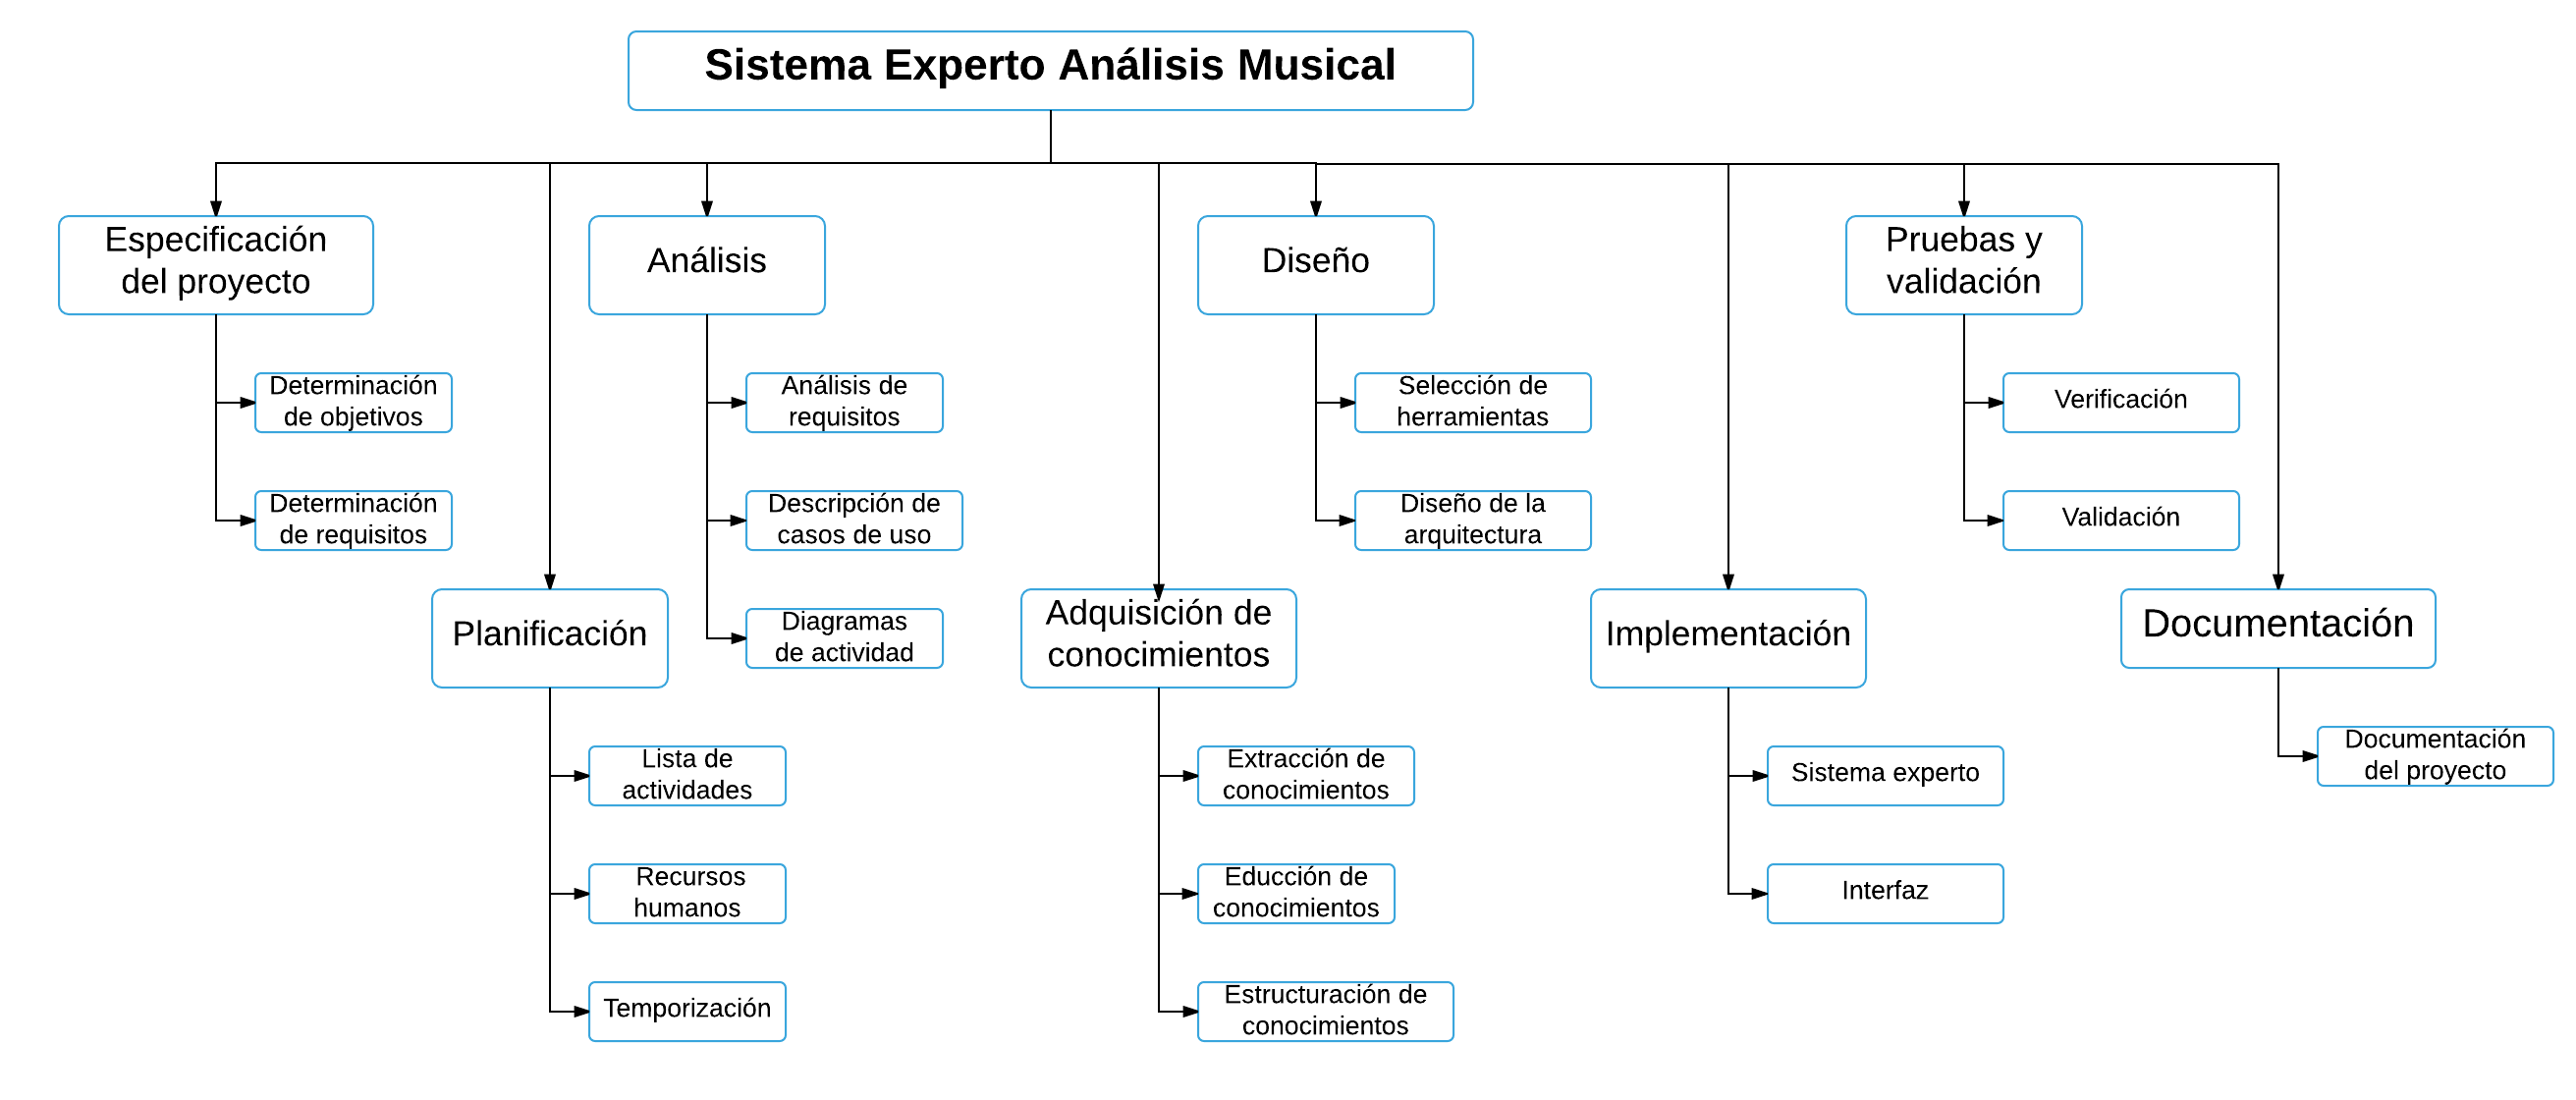
\includegraphics[scale=0.5]{imagenes/diagrama_edt.png}
	\caption{Diagrama de estructura de descomposición de trabajo}
	\label{fig1.4.1}
\end{figure}

\begin{figure}[H]
	\centering
	\hspace*{-0.6in}
	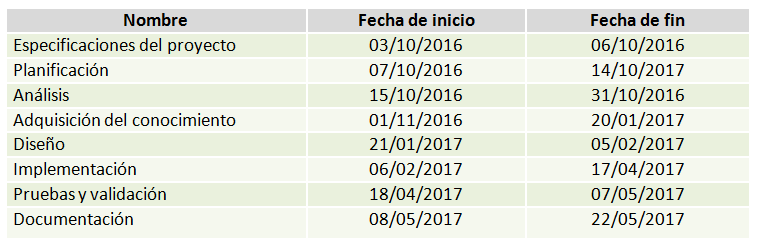
\includegraphics[scale=0.7]{imagenes/diagrama_tareas.png}
	\caption{Temporización de las tareas}
	\label{fig1.4.2}
\end{figure}

\bigskip
\bigskip

\begin{figure}[H]
	\centering
	\hspace*{-0.6in}
	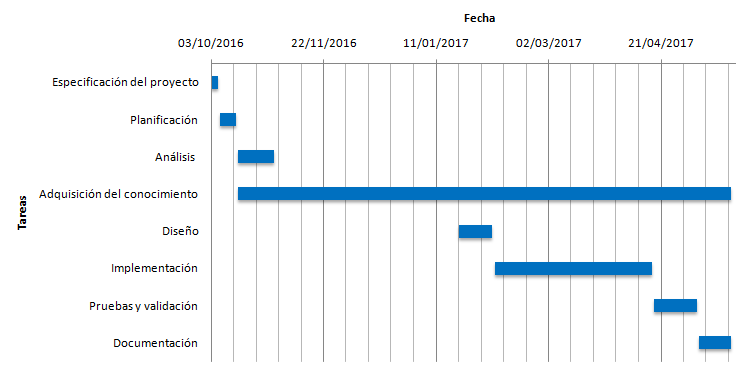
\includegraphics[scale=0.80]{imagenes/diagrama_gantt.png}
	\caption{Diagrama de Gantt}
	\label{fig1.4.3}
\end{figure}
\chapter{Análisis}

\section{Objetivos}

Los objetivos que se desean alcanzar con este sistema son los siguientes:

\bigskip
\textbf{OBJ-1.} El sistema deberá analizar una partitura en busca de faltas producidas por los movimientos de las voces.

\textbf{OBJ-2.} El sistema deberá analizar desde un punto e vista melódico una partitura y comprobar la existencia de errores referidos a la línea melódica y de contrapunto.

\textbf{OBJ-3.} El sistema deberá analizar desde un punto de vista armónico una partitura y comprobar la existencias de errores referidos a la armonía.

\textbf{OBJ-4.} El sistema mostrará todos los errores encontrados. 

\section{Análisis de requisitos}

La especificación de requisitos de un sistema experto comprende la determinación de requerimientos de información, funcionales y de entrada de datos. En esta fase del desarrollo debemos determinar qué datos de entrada, proporcionados por el usuario, necesita el sistema para funcionar, las operaciones que llevará a cabo sobre dichos datos y los resultados que espera obtener del sistema.  

Para poder realizar esta fase del desarrollo, necesitamos extraer esta serie de requisitos de los que serán los usuarios finales del sistema.

Como se menciona en la introducción, este sistema está dirigido a compositores o estudiantes de composición y armonía que desean mejorar sus obras o comprobar si éstas no contienen errores armónicos y/o melódicos. Éstos serían nuestros usuarios finales y a los que he consultado qué respuesta esperarían del sistema, es decir, qué elementos deberían analizarse en la partitura y cómo mostrar los posibles errores encontrados, así como qué información sería necesaria proporcionar para poder llevar a cabo el análisis deseado. 

\subsection{Actores}

Los actores implicados serán tres: el \textbf{ingeniero del conocimiento} y desarrollador, los \textbf{expertos} y los \textbf{usuarios} finales.

\begin{itemize}

	\item El \textbf{ingeniero del conocimiento} y desarrollador será el encargado de extraer y educir el conocimiento necesario para poder construir el sistema experto y llevar a cabo su implementación.

	\item Los \textbf{expertos} serán las personas que nos proporcionarán la principal fuente de conocimiento sobre el ámbito del problema a resolver por el sistema experto.	

	\item Los \textbf{usuarios} finales serán las personas a las que estará dirigido el sistema para su uso. Además, también serán una fuente de conocimiento para el sistema experto, concretamente sobre lo relacionado a los requisitos y funcionalidades del sistema.

\end{itemize}

\subsection{Requisitos de información}

\subsubsection{Requisitos de entrada de datos}

Los datos de entrada necesarios para el funcionamiento del sistema son las opciones de los distintos tipos de análisis posibles y la partitura en la que se van a realizar. 

Las opciones se mostrarían en un formulario multi-opción para permitir que el usuario pueda escoger una o varias según sus necesidades. 

El formato de la partitura sería xml. Esto se debe a que al ser un estándar permite trabajar con la partitura de forma más cómoda y sencilla facilitando en gran medida el desarrollo del sistema. Además, todos los editores de partituras permiten exportar a este formato, con lo que no supondría tampoco un incoveniente para los usuarios.

\begin{itemize}

	\bigskip
	\item \textbf{RI-1. PARTITURA.}
		\begin{itemize}
			\item Archivo que contiene la partitura de coro a analizar por el sistema.
			\item \textbf{Requisitos asociados}: RF-1, RF-2.
		\end{itemize}

	\bigskip
	\item \textbf{RI-2. OPCIONES DE ANÁLISIS.}
		\begin{itemize}
			\item Lista de opciones sobre los tipos de análisis posibles a realizar sobre la partitura en busca de errores.
			\item \textbf{Requisitos asociados}: RF-1, RF-2.
		\end{itemize}

\end{itemize}


\subsubsection{Requisitos de salida de datos}

El sistema, una vez finalizado el análisis, mostrará una lista seriada de los diferentes errores y faltas encontrados. Éstos estarán debidamente explicados y señalizados en la partitura, indicando las voces implicadas y el compás en el que aparecen. Dado que estos errores pueden ser de origen diverso - armónico o melódico - se crearán listados específicos para cada tipo de análisis, a fin de facilitar el entendimiento de los resultados y la experiencia del usuario.   


\begin{itemize}

	\bigskip
	\item \textbf{RI-3. FALTAS POR MOVIMIENTOS.}
		\begin{itemize}
			\item Lista de errores provocados por movimientos directos o paralelos de las voces.
			\item \textbf{Requisitos asociados}: RF-1.1, RF-1.2, RF-1.3, RF-1.4, RF-1.5, RF-1.6.
		\end{itemize}

	\bigskip
	\item \textbf{RI-4. ERRORES MELÓDICOS.}
		\begin{itemize}
			\item Lista de errores referidos al contrapunto y la dirección de las voces.
			\item \textbf{Requisitos asociados}: RF-2.
		\end{itemize}

	\bigskip
	\item \textbf{RI-5. ERRORES ARMÓNICOS.}
		\begin{itemize}
			\item Lista de errores referidos al mal uso de estructuras armónicas.
			\item \textbf{Requisitos asociados}: RF-1.7, RF-1.8, RF-1.9.
		\end{itemize}

\end{itemize}

\subsection{Requisitos funcionales}

El eje principal de este sistema radica en dos funciones principales: análisis armónico y análisis melódico.

La realización del análisis armónico implica la comprobación de los siguientes hechos:

\begin{itemize}

	\item \textit{Quintas paralelas}: dadas dos voces, éstas no pueden producir dos intervalos de quinta consecutivos. No obstante, si el segundo intervalo de quinta es de tipo aumentado o disminuido y no se encuentra en voces extremas no se considerará falta.

	\begin{figure}[H]
		\centering
		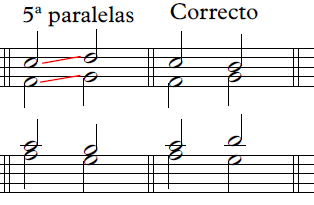
\includegraphics[scale=0.7]{imagenes/5paralelas.png}
		\caption{Ejemplo de quintas paralelas}
		\label{fig2.1.1}
	\end{figure}

	\item \textit{Quintas directas}: dadas dos voces, éstas no pueden producir un intervalo de quinta por movimiento directo.

	\begin{figure}[H]
		\centering
		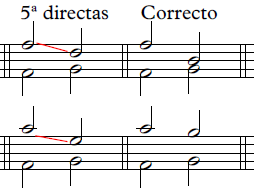
\includegraphics[scale=0.7]{imagenes/5directas.png}
		\caption{Ejemplo de quintas directas}
		\label{fig2.1.2}
	\end{figure}

	\item \textit{Octavas paralelas}: dadas dos voces, éstas no pueden producir dos intervalos de octava consecutivos. 

	\begin{figure}[H]
		\centering
		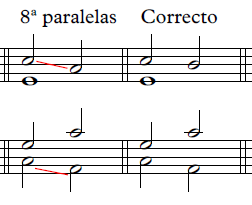
\includegraphics[scale=0.7]{imagenes/8paralelas.png}
		\caption{Ejemplo de octavas paralelas}
		\label{fig2.1.3}
	\end{figure}

	\item \textit{Octavas directas}: dadas dos voces, éstas no pueden producir un intervalo de octava por movimiento directo.

	\begin{figure}[H]
		\centering
		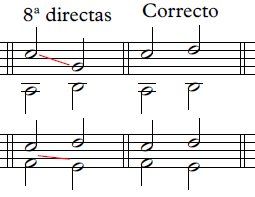
\includegraphics[scale=0.7]{imagenes/8directas.png}
		\caption{Ejemplo de octavas directas}
		\label{fig2.1.4}
	\end{figure}

	\item \textit{Tritono}: dadas dos voces, éstas no pueden producir un intervalo de cuarta aumentada o tritono. No obstante, si éste viene preparado por movimiento conjunto u oblicuo de las voces no se considerará falta.

	\begin{figure}[H]
		\centering
		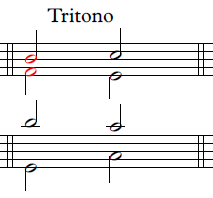
\includegraphics[scale=0.7]{imagenes/tritono.png}
		\caption{Ejemplo de cuarta aumentada}
		\label{fig2.1.5}
	\end{figure}

	\item \textit{Duplicación de sensible}: en ningún caso se podrá duplicar la sensible de la tonalidad. 

	\begin{figure}[H]
		\centering
		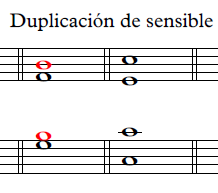
\includegraphics[scale=0.7]{imagenes/sensibledup.png}
		\caption{Ejemplo de duplicación de sensible}
		\label{fig2.1.6}
	\end{figure}

	\item \textit{Búsqueda de acordes incompletos}: todos los acordes deberán de tener la fundamental, la tercera y la quinta del acorde en al menos una voz, especialmente si están invertidos. No obstante, se puede dar la situación de que el acorde de tónica quede incompleto, con la ausencia de la quinta, en la cadencia.

	\item \textit{Segunda inverión consecutiva}: en ningún caso podrá haber dos acordes en segunda inversión consecutivos.

	\item \textit{Lógica tonal}: la armonía de la obra deberá seguir, en la medida de lo posible, el esquema indicado en la figura .

		\begin{itemize}

			\item La tónica o primer grado (I) podrá moverse hacia cualquier otro grado de la escala.
			\item La supertónica o segundo grado (II) podrá moverse hacia el cuarto, quinto o séptimo grado.
			\item La mediante, modal o tercer grado (III) podrá moverse hacia sexto grado.
			\item La subdominante o cuarto grado (IV) podrá moverse hacia el segundo, quinto o séptimo grado.
			\item La dominante o quinto grado (V) podrá moverse hacia el primer, sexto o séptimo grado.
			\item La superdominante o sexto grado (VI) podrá moverse hacia el segundo o cuarto grado.
			\item La subtónica o séptimo grado (VII) podrá moverse hacia el primer, tercer o quinto grado.
		\end{itemize}

		\begin{figure}[H]
			\centering
			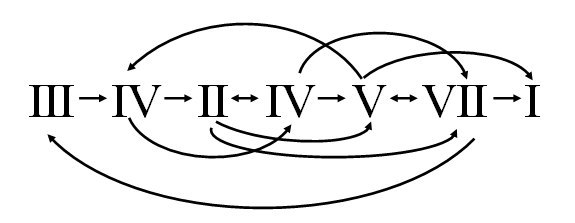
\includegraphics[scale=0.7]{imagenes/logica.jpg}
			\caption{Diagrama de lógica tonal}
			\label{fig2.1.7}
		\end{figure}

		Por otra parte, no podrán darse en ningún caso las siguientes sucesiones de acordes:

		\begin{itemize}
			\item I-II en estado fundamental.
			\item II-III en estado fundamental,
			\item III-IV en estado fundamental.
		\end{itemize}

\end{itemize}

\bigskip

La realización del análisis melódico implica la comprobación de los siguientes hechos:

\begin{itemize}

	\item \textit{Resolución de sensibles}: la sensible de la tonalidad deberá resolver siempre en la tónica.

	\begin{figure}[H]
		\centering
		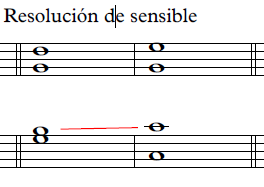
\includegraphics[scale=0.7]{imagenes/sensibleres.png}
		\caption{Ejemplo sensible sin resolver}
		\label{fig2.1.8}
	\end{figure}

	\item \textit{Resolución de séptimas}: la séptima de dominante deberá resolver siempre por movimiento por grado conjunto descendente y deberá estar preparada.

	\begin{figure}[H]
		\centering
		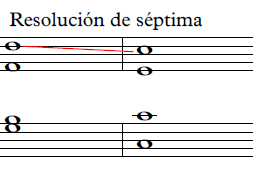
\includegraphics[scale=0.7]{imagenes/septimares.png}
		\caption{Ejemplo de séptima de dominante sin resolver}
		\label{fig2.1.9}
	\end{figure}

	\item \textit{Segunda aumentada}: en ningún caso podrá haber un intervalo de segunda aumentada entre dos notas consecutivas en una misma voz.

	\begin{figure}[H]
		\centering
		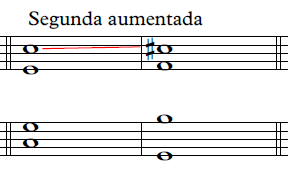
\includegraphics[scale=0.7]{imagenes/2aumentada.png}
		\caption{Ejemplo de segunda aumentada melódica}
		\label{fig2.1.10}
	\end{figure}

	\item \textit{Tritono melódico}: en ningún caso podrá haber un intervalo de cuarta aumentada o tritono entre dos notas consecutivas en una misma voz.

	\begin{figure}[H]
		\centering
		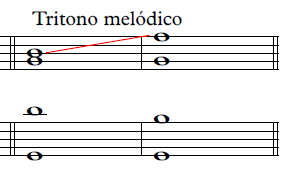
\includegraphics[scale=0.7]{imagenes/tritonomel.png}
		\caption{Ejemplo de cuarta aumentada melódica}
		\label{fig2.1.11}
	\end{figure}

	\item \textit{Contrapunto en voces extremas}: deberá predominar el movimiento contrario en las voces extremas sobre el movimiento oblicuo y, especialmente, directo.

	\item \textit{Contrapunto del salto}: si hay dos movimientos (saltos) en la misma dirección, ascendente o descendente, la primera y la última nota no pueden ser disonantes.

	\item \textit{Melodía incoherente}: deberá predominar el movimiento por grados conjuntos en las melodías, evitando hacer demasiados saltos.

\end{itemize}

\bigskip
\bigskip

En base a todas estas reglas los requisitos funcionales sería los siguientes:

\textbf{RF-1.}Análisis armónico. \\
El sistema llevará cabo un análisis sobre la armonía y los acordes de la partitura en busca de faltas y errores en las secuencias armónicas.

\begin{itemize}

	\bigskip
	\item \textbf{RF-1.1.} Se realizará la búsqueda de quintas paralelas.

	\bigskip
	\item \textbf{RF-1.2.} Se realizará la búsqueda de quintas directas.

	\bigskip
	\item \textbf{RF-1.3.} Se realizará la búsqueda de octavas paralelas.

	\bigskip
	\item \textbf{RF-1.4.} Se realizará la búsqueda de octavas directas.

	\bigskip
	\item \textbf{RF-1.5.} Se realizará la búsqueda de tritonos o cuartas aumentadas.

	\bigskip
	\item \textbf{RF-1.6.} Se realizará la búsqueda de sensibles duplicadas.

	\bigskip
	\item \textbf{RF-1.7.} Se realizará la búsqueda de acordes incompletos.

	\bigskip
	\item \textbf{RF-1.8.} Se realizará la búsqueda de secuencias de acordes en segunda inversión consecutivos.

	\bigskip
	\item \textbf{RF-1.9.} Se realizará una comprobación sobre las secuencias de acordes para asegurar que siguen las reglas de la lógica tonal.

\end{itemize}

\bigskip
\textbf{RF-2.} Análisis melódico.\\
El sistema llevará a cabo un análisis sobre las melodías de las voces en busca de una mala conducción de éstas o de un mal uso del contrapunto.

\begin{itemize}

	\bigskip
	\item \textbf{RF-2.1.} Se comprobará la resolución de sensibles en la tónica.

	\bigskip
	\item \textbf{RF-2.2.} Se comprobará la resolución de todas las séptimas de dominante.

	\bigskip	
	\item \textbf{RF-2.3.} Se comprobará la existencia de intervalos de segunda aumentada melódicos.

	\bigskip
	\item \textbf{RF-2.4.} Se comprobará la existencia de tritonos o intervalos de cuarta aumentada melódicos.

	\bigskip
	\item \textbf{RF-2.5.} Se comprobará la existencia de un buen contrapunto entre las voces de la soprano y del bajo.

	\bigskip
	\item \textbf{RF-2.6.} Se comprobará la existencia de saltos consecutivos con disonancias.

	\bigskip
	\item \textbf{RF-2.7.} Se comprobará la existencia de una buena praxis en las líneas melódicas. 

\end{itemize}

\subsection{Requisitos no funcionales}

Los requisitos no funcionales son aquellos referidos al desarrollo pero no necesariamente relacionados con la funcionalidad del sistema, como aspectos referidos a la interfaz, al rendimiento o a la fiabilidad del sistema.

\bigskip
\textbf{RNF-1.} Los usuarios del sistema deberán estar familiarizados con el lenguaje específico empleado en el ámbito musical para poder entender las explicaciones aportadas por el sistema.

\textbf{RNF-2.} Las pruebas y validaciones del sistema se llevarán a cabo por uno de los expertos.

\section{Modelos de casos de uso}

\subsection{Descripción básica de los actores}

\begin{table}[H]
	\begin{tabular}{@{}|l|p{9cm}|p{2cm}|@{}}
		\hline
		\textbf{Actor}  & Ingeniero del conocimiento & \cellcolor[HTML]{C0C0C0}ACT-1  \\ \hline
		\textbf{Descripción} & \multicolumn{2}{p{11cm}|}{Ingeniero encargado del proceso de adquisición de conocimiento y creación del sistema} \\ \hline
		\textbf{Características} & \multicolumn{2}{p{11cm}|}{Es también el desarrollador que lleva a cabo la implementación del sistema.} \\ \hline
		\textbf{Relaciones} & \multicolumn{2}{p{11cm}|}{ACT-2, ACT-3} \\ \hline
		\textbf{Referencias} & \multicolumn{2}{p{11cm}|}{} \\ \hline
	\end{tabular}
	\caption{Descripción del actor Ingeniero del Conocimiento}
	\label{tablaACT1}
\end{table}

\begin{table}[H]
	\begin{tabular}{@{}|l|p{9cm}|p{2cm}|@{}}
		\hline
		\textbf{Actor} & Experto & \cellcolor[HTML]{C0C0C0}ACT-2 \\ \hline
		\textbf{Descripción} & \multicolumn{2}{p{11cm}|}{Persona a la que el ingeniero del conocimiento entrevista para conocer el ámbito del problema y los procedimientos necesarios para su resolución} \\ \hline
		\textbf{Características} & \multicolumn{2}{p{11cm}|}{Persona experta en el ámbito del problema a resolver por el sistema experto.} \\ \hline
		\textbf{Relaciones} & \multicolumn{2}{p{11cm}|}{ACT-1} \\ \hline
		\textbf{Referencias} & \multicolumn{2}{p{11cm}|}{} \\ \hline
	\end{tabular}
	\caption{Descripción del actor Experto}
	\label{tablaACT2}
\end{table}

\begin{table}[H]
	\begin{tabular}{@{}|l|p{9cm}|p{2cm}|@{}}
		\hline
		\textbf{Actor} & Usuario & \cellcolor[HTML]{C0C0C0}ACT-3 \\ \hline
		\textbf{Descripción} & \multicolumn{2}{p{11cm}|}{Usuario final al que está dirigido el sistema} \\ \hline
		\textbf{Características} & \multicolumn{2}{p{11cm}|}{El usuario, al igual que el experto, tendrá algunos conocimientos sobre el dominio del problema} \\ \hline
		\textbf{Relaciones} & \multicolumn{2}{p{11cm}|}{ACT-1} \\ \hline
		\textbf{Referencias} & \multicolumn{2}{p{11cm}|}{} \\ \hline
	\end{tabular}
	\caption{Descripción del actor Usuario}
	\label{tablaACT3}
\end{table}

\subsection{Descripción de casos de uso}

\begin{table}[H]
	\begin{tabular}{@{}|l|p{9cm}|p{2cm}|@{}}
		\hline
		\textbf{Caso de uso} & Analizar partitura & \cellcolor[HTML]{C0C0C0}CU-1 \\ \hline
		\textbf{Actores} & \multicolumn{2}{p{11cm}|}{Usuario} \\ \hline 
		\textbf{Tipo} & \multicolumn{2}{p{11cm}|}{Primario, esencial.} \\ \hline
		\textbf{Referencias} & \multicolumn{2}{p{11cm}|}{RI-1,RI-2,,RI-3,RI-4,RI-5,RF-1,RF-2} \\ \hline
		\textbf{Precondición} & \multicolumn{2}{p{11cm}|}{Partitura almacenada en el servidor y opciones seleccionadas enviadas} \\ \hline
		\textbf{Postcondición} & \multicolumn{2}{p{11cm}|}{Se crearán archivos con los resultados del análisis para mostrarse a través de la interfaz.} \\ \hline
		\textbf{Propósito} & \multicolumn{2}{p{11cm}|}{Realización del análisis deseado en la partitura aportada por el usuario y obtenicón de resultados.} \\ \hline
		\textbf{Resumen} & \multicolumn{2}{p{11cm}|}{Una vez se han propocionado todos los datos necesarios, el usuario podrá activar el sistema para obtener la lista de errores y faltas encontrados en su partitura para su posterior corrección.} \\ \hline
	\end{tabular}
	\caption{Descripción del caso de uso CU-1}
	\label{CU-1}
\end{table}

\begin{table}[H]
	\begin{tabular}{@{}|p{7.1cm}|p{7.1cm}|@{}}
		\hline
		\multicolumn{2}{|c|}{\textbf{Curso normal}}\\ \hline
		{Accion del actor} & {Acción del sistema} \\ \hline
		(1) Usuario: selecciona las opciones de análisis propuestas por el sistema. & \\ \hline
		 & (2) Sistema: comprueba las opciones seleccionadas. \\ \hline 
		(3) Usuario: selecciona el archivo de la partitura y lo sube al servidor del sistema. &  \\ \hline
		 & (3) Sistema: comprueba el archivo adjuntado.  \\ \hline 
		(5) Usuario: envía los datos al sistema. & \\ \hline
		 & (6) Sistema: almacena las opciones seleccionadas por el usuario.  \\ \hline
		 & (7) Sistema: almacena la partitura en el servidor.  \\ \hline
		 & (8) Sistema: lanza los módulos de análisis seleccionados.  \\ \hline
		 & (9) Sistema: obtiene los resultados de los módulos. \\ \hline
		 & (10) Sistema: muestra los resultados de los módulos. \\ \hline
	\end{tabular}
	\caption{Descripción del curso normal del caso de uso CU-1}
	\label{CNCU-1}
\end{table}

\begin{table}[H]
	\begin{tabular}{@{}|p{14.7cm}|@{}}
		\hline
		\textbf{Cursos alternos}\\ \hline
		(2a) El usuario no ha seleccionado ninguna opción. \\ 
		\hspace{1.5cm}Sistema: informa del error y vuelve a solicitar la selección de opciones. \\
		(4a) El usuario no ha seleccionado ningún archivo. \\
		\hspace{1.5cm}Sistema: informa del error y vuelve a solicitar la selección de un archivo. \\
		(4b) El usuario ha seleccionado un archivo no válido. \\
		\hspace{1.5cm}Sistema: informa del error y vuelve a solicitar la selección de un archivo válido. \\ \hline
	\end{tabular}
	\caption{Descripción de los cursos alternos del caso de uso CU-1}
	\label{CACU-1}
\end{table}

%\section{Diagramas de casos de uso}

%\begin{figure}[H]
%	\centering
%	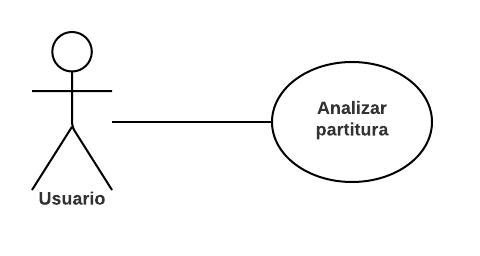
\includegraphics[scale=0.7]{imagenes/casoUso.png}
%	\caption{Diagrama de casos de uso}
%	\label{fig2.4.1}
%\end{figure}

\section{Diagramas de actividad}

\begin{figure}[H]
	\centering
	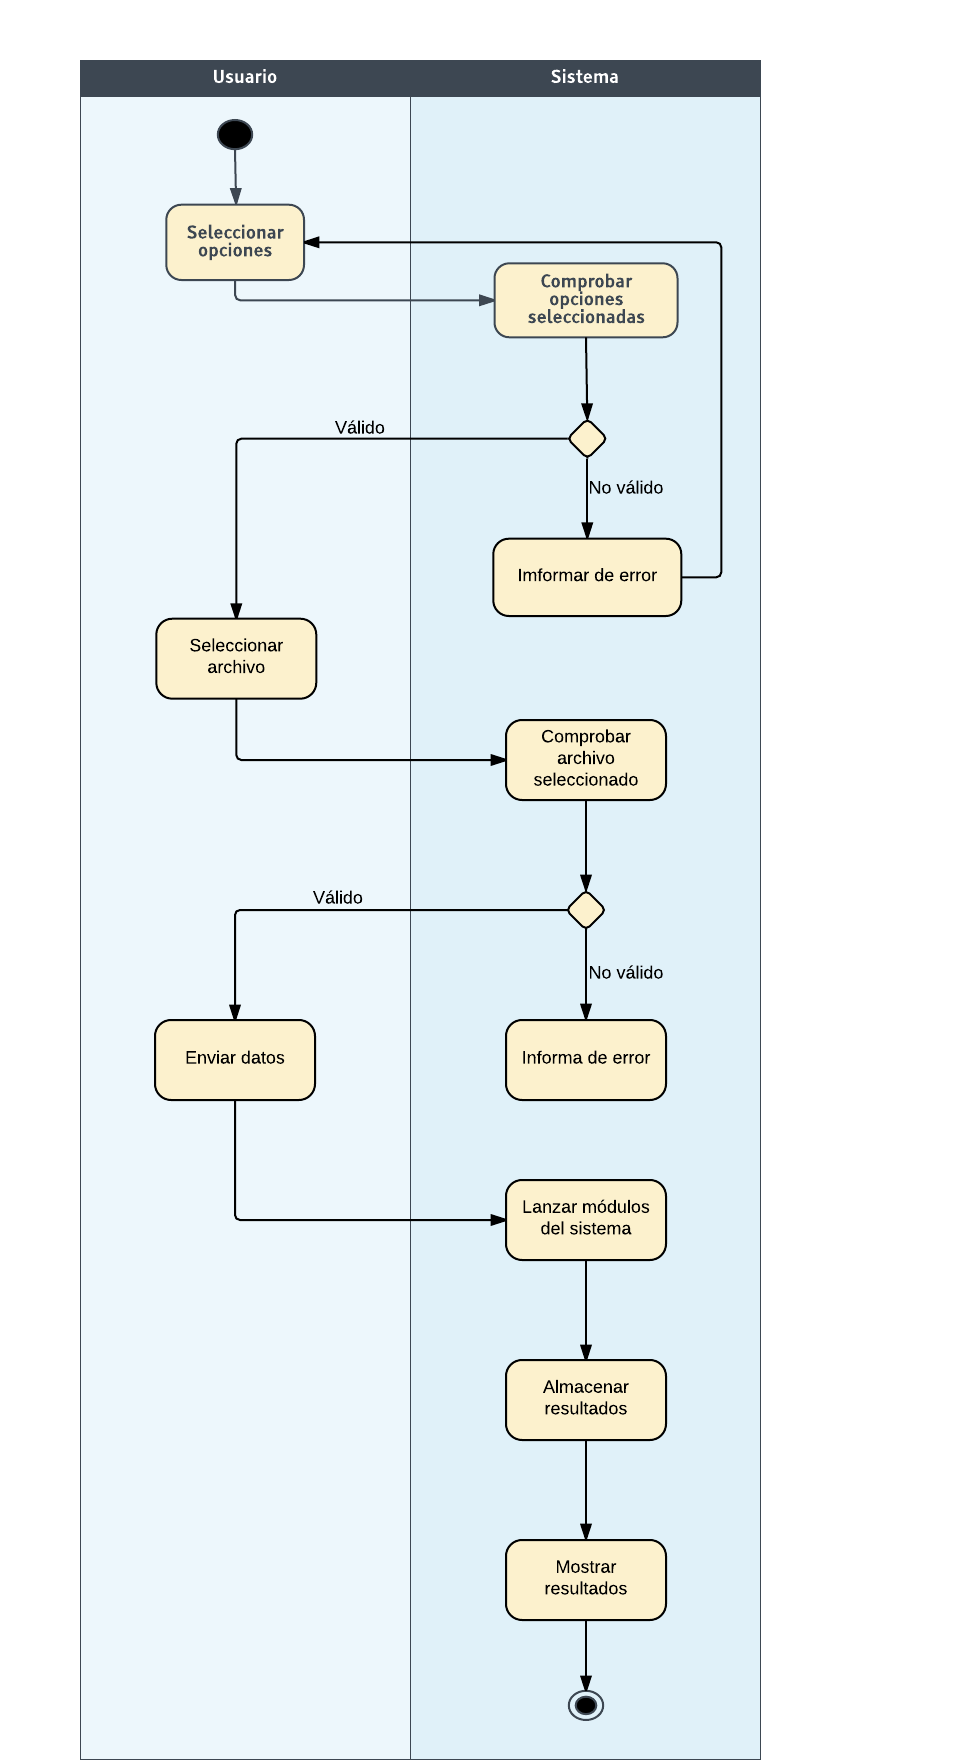
\includegraphics[scale=0.65]{imagenes/diagramaAct.png}
	\caption{Diagrama de actividad del caso de uso CU-1. Analizar partitura.}
	\label{fig2.5.1}
\end{figure}
\chapter{Adquisión de conocimiento}

La adquisición y educción del conocimiento constituye una de las fases más importantes del desarrollo de este tipo de sistemas. En esta etapa es donde el Ingeniero del Conocimiento interactúa con el experto para obtener la información sobre la solución de los problemas, así como las estrategias utilizadas para la obtención de cada solución. Además de consultar con el experto, también se adquiere conocimiento de otras fuentes como libros, tratados, estudios, etc. Este proceso supone el ``cuello de botella'' del desarrollo.
 
Esta tarea no es un paso concreto en la metodología de desarrollo, sino que se va produciendo en paralelo al resto de etapas de construcción del sistema.

El proceso de adquisión de conocimiento se ha llevado a cabo en tres fases: 

\begin{itemize}
	\item Extracción de conocimientos
	\item Educción de conocimientos
	\item Estructuración de conocimientos
\end{itemize}
 
Para llevar a cabo estas tareas, he consultado a los expertos Alberto José Moreno Montes e Isabel Salado Ortega, ambos músicos titulados.  

\section{Extracción de conocimientos}

En la realización de esta tarea, se pretende aprender sobre el dominio tanto como sea posible antes de comenzar las sesiones con los expertos para facilitar la educción de conocimientos. 

Al haber estudiado música en el conservatorio hace algunos años, esta fase supuso más bien un proceso de recordar que de aprender. No obstante, al ser un dominio tan extenso, es necesario consultar la documentación adecuada y más útil para la aplicación a nuestro problema. Por este motivo, pregunté a ambos expertos, Alberto e Isabel, sobre el material más importante a consultar, incluyendo libros, manuales y tratados. Las dos fuentes más relevantes y de las cuáles se extrajo la mayoría de conocimientos previos fueron el \textit{Tratado de Armonía}, vólumenes I y II,de Joaquín Zamacois \cite{ZAMACOIS1, ZAMACOIS2} y \textit{Armonía} por Walter Piston \cite{PISTON}. Ambos se incluyen, junto con el resto de fuentes, en las referencias bibliográficas. 

De estos libros se determinaron la mayoría de definiciones y conceptos generales sobre lenguaje musical y armonía.

\section{Educción de conocimientos}

Gracias a los conocimientos adquiridos en la fase anterior, realizamos una serie de entrevistas estructuradas con los expertos. En estas entrevistas se formularon cuestiones concretas y previamente planificadas con el fin de educir conocimiento de una forma más eficiente. Nos centramos en definir conceptos específicos y procedimientos necesarios a la hora de analizar partituras, haciendo especial énfasis en el análisis melódico, el cual tiende a ser más delicado de realizar y con un componente subjetivo más fuerte.

La mayor dificultad de este proceso radicó en la cantidad de situaciones excepcionales que pueden darse y de la subjetividad que viene adherida a cualquier arte. Por ejemplo, las excepciones a la falta de \textit{quintas paralelas}. Las \textit{quintas paralelas} son una de las faltas más graves, dado que al darse se produce una sonoridad más dura y arcaica. Sin embargo, éstas pueden permitirse si la segunda quinta que se forma es una quinta disminuida, salvo que ésta se forme con el bajo o en voces extremas, en cuyo caso se considerará falta.

Como podemos observar en este ejemplo, las reglas armónicas no son directrices sencillas de llevar a cabo o entender fácilmente. Con el fin de poder comprenderlas empleé con Alberto e Isabel lo que denominamos ``incidentes críticos''. 

\subsection{Incidentes críticos}
 
Con la técnica de ``incidentes críticos'', ambos expertos me describieron los casos excepcionales mencionados anterioremente y algunas de las dificultades más relevantes a la hora de realizar un análisis armónico y/o melódico. 

Me explicaron todas las posibles excepciones para cada regla, ejemplificándome cada una de las situaciones. 

En el caso de los problemas derivados por la subjetividad a la hora de analizar las melodías de un coral, Alberto sugirió ceñirse lo más posible al estilo de los corales compuestos durante la época barroca, ya que las restricciones a la hora de componer eran más fuertes y estaban mejor delimitadas.  

\section{Estructuración de conocimientos} 

Una vez hemos finalizado la extracción y la educción de conocimientos pasamos a analizar, organizar y estructurar todos los conocimientos obtenidos para crear nuestra base de conocimiento.

En un primer paso, constrastamos toda la información que hemos adquirido junto con los requisitos del sistema para filtrar qué conocimientos son los necesarios y útiles para poder llevar a cabo los distintos análisis en el coral. Los tipos de análisis son independientes entre sí, por lo que se hizo una filtración de información para cada uno de ellos. Aunque el tener distintos análisis sobre la partitura podía suponer una dificultad para este proceso de selección, el hecho de ser independientes supuso una gran ventanja, facilitándolo en gran medida. 

A continuación, organizamos y estructuramos el conocimiento diviéndolo en \textit{hechos} y \textit{reglas}. 

\begin{itemize}

	\item Los \textit{hechos} serán asertados en el sistema. Para definir la mayoría de estos hechos se hará uso de estructuras ``\texttt{templates}'' o plantillas.

	\bigskip

		\begin{lstlisting}

			(intervalo (distancia d) (tipo t) (nota1 n1) (nota2 n2))

		\end{lstlisting}

	\bigskip

	\item Las \textit{reglas} definirán los requisitos funcionales del sistema en forma de estructuras \textit{si <<antecedente>> entonces <<consecuente>>}. 

	\bigskip

		\begin{lstlisting}

			if intervalo.distancia = 2 then intervalo.tipo = disonante

		\end{lstlisting}

	\bigskip

\end{itemize} 

Este conjunto de hechos y reglas constituirá la base de conocimiento del sistema experto. Estas reglas utilizarán los hechos almacenados en la base de conocimiento, junto con los hechos calculados a partir de los datos de entrada, para deducir nuevos hechos y conocimientos que permitan obtener conclusiones finales y así obtener resultados.

\subsection{Hechos}

Los hechos del sistema se dividen en tres tipos:

\begin{itemize}

	\item \textbf{Hechos asertados}: son los hechos que constituyen la base de conocimiento ``inicial'' del sistema. Estos hechos constituyen todo el conocimiento necesario ,referido principalmente a conceptos, para poder analizar una partitura. 

	\item \textbf{Hechos calculados}: son los hechos que extraemos directamente de la partitura, es decir, las notas que la componen con sus alteraciones, su altura y su duración.

	\item \textbf{Hechos deducidos}: son los hechos que el sistema deduce aplicando las reglas a los hechos asertados y calculados. También puede deducir hechos a partir de hechos previamente deducidos que sea utilizados por las reglas.

\end{itemize}

\bigskip

Los hechos asertados están referidos a los siguientes conceptos:

\begin{itemize}

	\item \textit{Tonalidades}: todas las posibles tonalidades existentes indicando el nombre de la tonalidad, el modo, las alteraciones que tienen en su armadura y la sensible.

	\begin{lstlisting}

		(tonalidad (nombre D) (tipo mayor) (armadura 2s) (sensible Cs))

	\end{lstlisting}

	Las tonalidades las usaremos para poder determinar qué tipo de alteraciones tienen las notas de la partitura por defecto y cuáles serían alteraciones accidentales. También nos indican la sensible de la tonalidad, la cuál usaremos para comprobar varios errrores.

	\bigskip

	\item \textit{Escalas}: todas las escalas mayores y menores asociadas a cada tonalidad, indicando el nombre de la escala y las notas (grados) que la componen. 

	\begin{lstlisting}

		(escala (nombre D) (tipo mayor) (grado_I G) (grado_II A) (grado_III B) (grado_IV C) (grado_V D) (grado_VI E) (grado_VII Fs))

	\end{lstlisting}

	A partir de la escala podemos deducir todos los acordes fundamentales de la tonalidad. Con ellos realizaremos el análisis armónico comprobando acordes incompletos, sucesiones erróneas, etc.

	\bigskip

	\item \textit{Intervalos}: todos los tipos de intervalos desde segundas menores hasta octavas justas desde cada una de las posibles notas. Indicamos la distancia, el tipo y las dos notas que lo forman.

	\begin{lstlisting}

		(intervalo (distancia 3) (tipo mayor) (nota1 G) (nota2 B))

	\end{lstlisting}

	Necesitamos conocer todos los intervalos posibles para poder evaluar saltos y contrapunto en las melodías, así como movimientos armónicos entre las voces, como las quintas paralelas u octavas entre otras faltas.

	\bigskip

	\item \textit{Acordes}: todos los acordes de cada uno de los grados de cada tonalidad. Los acordes pueden ser de tríada (formados por tres notas) o cuatríada (formados por cuatro notas), por lo que diferenciamos ambos tipos. Indicamos el grado de la escala a partir de la cuál se forma el acorde, el nombre y el modo de la tonalidad a la que pertenece y las notas que lo componen: fundamental, tercera y quinta en el caso de acordes de tríada y fundamental, tercera, quinta y séptima en el caso de acordes de cuatríada.

	\begin{lstlisting}

		(acorde_3 (grado I) (nombre_tonalidad C) (modo_tonalidad mayor) (fundamental C) (tercera E) (quinta G))

	\end{lstlisting}

	\begin{lstlisting}

		(acorde_4 (grado V) (nombre_tonalidad C) (modo_tonalidad mayor) (fundamental G) (tercera B) (quinta D) (septima F))

	\end{lstlisting}

	Los acordes los utilizaremos para poder realizar el análisis armónico.

	\bigskip

	\item \textit{Sucesiones lógicas}: lista de sucesiones permitidas entre acordes según las normas de la armonía tradiciones. Se indican los dos grados que componen una sucesión lógica.

	\begin{lstlisting}

		(sucesion_logica (grado1 V) (grado2 I))

	\end{lstlisting} 

	Esto nos permite analizar la coherencia armónica de la obra, es decir, que la estructura armónica sobre la que se construye el coral sea correcta y tenga una buena sonoridad.

\end{itemize}

\bigskip

Los hechos calculados del sistema son aquellos que extraemos a partir de la información contenida en la partitura.

\begin{itemize}

	\item Tonalidad: se extrae la tonalidad de la obra para poder determinar sobre qué escala tenemos que trabajar y qué acordes son los que vamos a analizar.

	\item Compás: se extrae el compás para poder localizar los errores.

	\item Notas: se extrae la información sobre las notas de la partitura. Dependiendo de si se va a realizar un análisis melódico o armónico extraeremos dos listas distintas de notas.

	\item Movimientos: se extrae también información sobre los movimientos de las notas para poder analizar tanto errores armónicos como melódicos.

\end{itemize}

\bigskip

Toda la información referida a estos hechos se explicará con más detalle en el apartado de la implementación.

\bigskip

Poŕ último, los hechos deducidos serán los que irá asertando el sistema tras aplicar reglas y utilizará para ir deduciendo nuevos hechos hasta llegar a las conclusiones finales, que en este caso serán la existencia o no de errores y faltas.

\subsection{Reglas}

Las reglas del sistema coinciden prácticamente con los requisitos funcionales descritos en el capítulo anterior, aunque para poder implementar algunas de estas reglas ha sido necesario añadir reglas auxiliares.

\begin{itemize}

	\item \textit{Reglas para cargar los hechos iniciales}: debido a varios problemas con la implementación, que se comentarán en el capítulo 5, los hechos asertados comentados en el apartado anterior serán asertados a partir de unas reglas que los cargarán en la memoria de trabajo. 

	\bigskip

	\item \textit{Reglas para la lectura de los datos extraídos de la partitura}: a continuación cargamos los hechos calculados. Estos son la información referida a las notas de la partitura, que ha sido previamente procesada para facilitar la aserción de estos hechos.
 
	\bigskip

	\item \textit{Reglas para detección de quintas}: este conjunto de reglas se encarga de detectar errores de quintas paralelas y quintas directas, teniendo en cuenta posibles casos excepcionales.

	\bigskip

	\item \textit{Reglas para detección de octavas}: detectan errores de octavas paralelas y octavas directas, comprobando posibles casos excepcionales.

	\bigskip

	\item \textit{Reglas para detección de tritonos armónicos}: comprueban si se da alguna el intervalo de cuarta aumentada entre dos voces, teniendo en cuenta la excepción de si está o no preparado.

	\bigskip

	\item \textit{Regla para comprobar la dulpicación de sensible}: comprueba que la sensible no se encuentre duplicada en dos voces bajo ninguna circunstancia.

	\bigskip

	\item \textit{Regla para comprobar la resolución de sensible}: esta regla comprueba que la sensible resuelva correctamente en la tónica de la tonalidad.

	\bigskip

	\item \textit{Regla para comprobar la resolución de séptima}: al igual que en el caso de la sensible, se comprueba que la séptima también resuelva correctamente, sin tener en cuenta ninguna resolución excepcional.

	\bigskip

	\item \textit{Reglas para comprobar tritonos y segundas aumentadas melódicas}: estas reglas comprueban que no se produzcan este tipo de intervalos en la melodía de ninguna voz.

	\bigskip

	\item \textit{Reglas para comprobar el contrapunto en voces extremas}: este conjunto de reglas analiza los movimientos de las melodías de la soprano y el bajo para comprobar que predomina el movimiento contrario u oblicuo sobre el movimiento directo entre las voces.

	\bigskip

	\item \textit{Reglas para comprobar el contrapunto del salto}: este conjunto de reglas realiza una función similar al contrapunto de voces extremas, pero se centra en cada línea melódica. Se comprueba que no se den saltos que puedan provocar disonancias.

	\bigskip

	\item \textit{Reglas para comprobar las líneas melódicas}: estas reglas analizan los movimientos de las voces respecto a si se hacen demasiados saltos grandes o predomina el movimiento por grado conjunto en las melodías. Con esto podemos determinar si una melodía está bien construida o por el contrario no tiene coherencia melódica.

	\bigskip

	\item \textit{Reglas para analizar acordes}: se analizan armónicamente el coral determinando su estructura armónica. Se consideran tanto acordes de tríada como acordes con séptima teniendo en cuenta sus posibles inversiones.

	\bigskip

	\item \textit{Reglas para analizar la lógica tonal}: a partir del análisis previo de los acordes, se comprueba que las sucesiones de éstos sean correctas y sigan patrones armónicos tradicionales.

	\bigskip

	\item \textit{Reglas para comprobar los acordes}: este conjunto de reglas comprueba que todos los acordes estén completos, es decir, que no falte ninguna de las notas que lo componen por hacer una mala duplicación de las notas en las voces. 

	\bigskip

	\item \textit{Reglas para mostrar los errores}: una vez detectados todos los errores con las reglas anteriores, implementamos una serie de reglas para poder mostrar los errores al usuario. Cada error se muestra debidamente explicado y localizado en la partitura.

\end{itemize}

\bigskip

\subsection{Estructura}

En total el sistema está compuesto por 873 hechos iniciales, previamente asertados, y 174 reglas. Hay que tener en cuenta que estos hechos iniciales son los hechos asertados, sin tener en cuenta todos los hechos que serán extraídos de la partitura. Dependiendo de la longitud del coral, se asertarán más o menos hechos calculados. Podemos estimar la cantidad de hechos calculados referidos a las notas de la siguiente manera:

\begin{itemize}

	\item Si el compás es binario:
		$$hechos\_calculados\_notas = n^{\circ}\ de\ partes\ del\ compas \times 16 \times n^{\circ}\ de\ compases$$

	\item Si el compás es ternario:
		$$hechos\_calculados\_notas = n^{\circ}\ de\ partes\ del\ compas \times 8 \times n^{\circ}\ de\ compases$$

\end{itemize}

\bigskip

Para hacernos una idea más exacta, si nuestro coral tiene 24 compases y un compás \lilyTimeSignature{4}{4} (compás binario de cuatro partes) en total tendríamos de 1536 hechos referidos únicamente a las notas. Tenemos que tener en cuenta que estos serían utilizados únicamente para realizar el análisis armónico. Para realizar el análisis melódico necesitamos el número de notas de cada voz, que dependerá del coral y no podemos conocer su número a priori. Además, tenemos otra serie de hechos calculados como los movimientos de las notas, que serán iguales a la cantidad de notas para el análisis melódico.

Esto significa que para analizar de manera completa un coral de la misma longitud y compás que el del ejemplo anterior y suponiendo que sea un coral sencillo sin demasiadas notas, vamos a suponer tres notas por compás en cada voz, contaríamos con cerca de 3000 hechos inicales.

Para facilitar la implementación y hacerlo más usable, como se ha comentado anteriormente, el sistema estará formado por varios módulos. A continuación se muestra un listado de los módulos indicando los hechos y reglas que los componen y el número de estos, sin tener en cuenta el número de hechos calculados que dependerán de la partitura:

\begin{itemize}

	\item \textbf{Módulo 1}: 408 hechos y 42 reglas.

	\begin{itemize}

		\item Hechos asertados:

			\begin{itemize}

				\item Tonalidades

				\item Intervalos

			\end{itemize}

		\item Hechos calculados:

			\begin{itemize}

				\item Tonalidad de la obra

				\item Compás

				\item Lista de notas de las voces para análisis armónico

				\item Lista de los movimientos de las melodías

			\end{itemize}

		\item Reglas:

			\begin{itemize}

				\item Reglas para cargar hechos iniciales

				\item Reglas para cargar hechos calculados

				\item Reglas para errores de quintas

				\item Reglas para errores de octavas

				\item Reglas para tritonos armónicos

				\item Regla para duplicación de sensible

				\item Reglas para mostrar errores

			\end{itemize}

	\end{itemize}

	\bigskip

	\item \textbf{Módulo 2}: 858 hechos y 82 reglas.

	\begin{itemize}

		\item Hechos asertados:

			\begin{itemize}

				\item Tonalidades

				\item Intervalos

				\item Escalas

				\item Acordes

			\end{itemize}

		\item Hechos calculados:

			\begin{itemize}

				\item Tonalidad de la obra

				\item Compás

				\item Lista de notas de las voces

				\item Lista de los movimientos de las melodías

			\end{itemize}

		\item Reglas:

			\begin{itemize}

				\item Reglas para cargar hechos iniciales

				\item Reglas para cargar hechos calculados

				\item Regla para resolución de sensible

				\item Regla para resolución de séptima

				\item Reglas para intervalos disonantes melódicos

				\item Reglas para contrapunto en voces extremas

				\item Reglas para contrapunto del salto

				\item Reglas para comprobar líneas melódicas

				\item Reglas para mostrar errores

			\end{itemize}
			
	\end{itemize}

	\bigskip

	\item \textbf{Módulo 3}: 875 hechos y 50 reglas.

	\begin{itemize}

		\item Hechos asertados:

			\begin{itemize}

				\item Tonalidades

				\item Intervalos

				\item Escalas

				\item Acordes

				\item Lógica tonal

			\end{itemize}

		\item Hechos calculados:

			\begin{itemize}

				\item Tonalidad de la obra

				\item Compás

				\item Lista de notas de las voces para análisis armónico

			\end{itemize}

		\item Reglas:

			\begin{itemize}

				\item Reglas para cargar hechos iniciales

				\item Reglas para cargar hechos calculados

				\item Regla para analizar acordes

				\item Regla para comprobar la lógica tonal

				\item Reglas para buscar acordes incompletos

				\item Reglas para mostrar errores

			\end{itemize}
			
	\end{itemize}

\end{itemize}

\bigskip

Como se puede observar, el sistema consta de una base inicial de conocimiento bastante compleja y amplia, aún sin tener en cuenta el conocimiento que nos aporta la partitura, el cuál aumenta aún más la complejidad del problema. También debemos tener en cuenta la cantidad de hechos deducidos a partir de las reglas, pero está dependerá de la cantidad de errores y faltas que haya en la partitura. 

\bigskip

En la siguiente figura se muestra un diagrama de la estructura del sistema experto para facilitar su comprensión:

\begin{figure}[H]
	\centering
	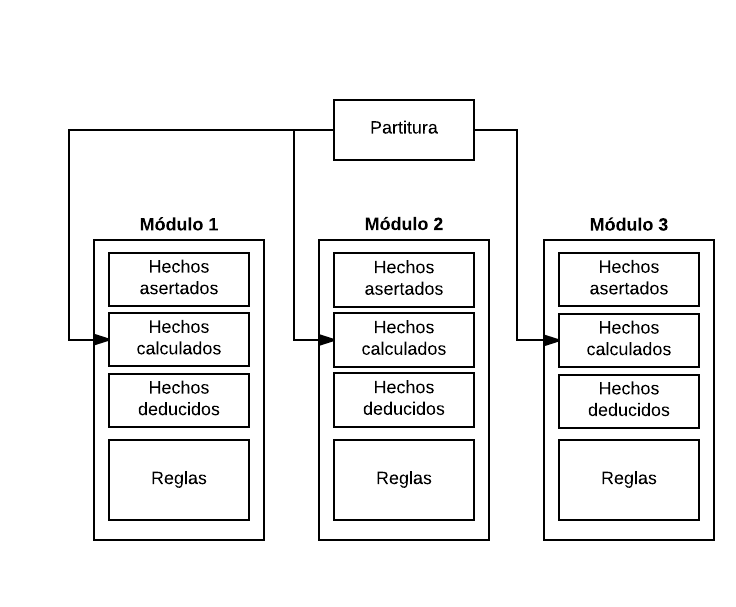
\includegraphics[scale=1]{imagenes/estructuraExp.png}
	\caption{Diagrama de la estructura del sistema experto}
	\label{fig3.1}
\end{figure}
\chapter{Diseño}

\section{Selección de herramientas}

\subsection{Sistema experto}

Para la implementación del sistema experto se consideraron las siguientes opciones:

\begin{itemize}

	\item \textbf{SWI-PROLOG}. Lenguaje basado en lógica y programación declarativa caracterizado por su capacidad de manipulación simbólica.

	\item \textbf{Expert System Builder}. Programa gratuito, implementado en Common Lisp, destinado a simplificar el desarrollo de sistemas expertos.

	\item \textbf{CLIPS}. Lenguaje basado reglas para desarrollar sistemas expertos. Basado en el lenguaje C para permitir una mayor portabilidad. 

\end{itemize} 

La herramienta Expert System Builder se desestimó al estar orientada al desarrollo de sistemas expertos para la toma de decisiones de una organización. 

La decisión entre escoger CLIPS o SWI-PROLOG se determinó por los siguientes factores:

\begin{itemize}

	\item CLIPS utiliza encadenamiento hacia delante y SWI-PROLOG encadenamiento hacia atrás. Los lenguajes que emplean encadenamiento hacia delante son más rápidos en el proceso de deducción, lo cuál hace que CLIPS sea más rápido en la ejecución de reglas que SWI-PROLOG.

	\item CLIPS se basa en el lenguaje C, el cuál sabemos es uno de los más eficientes en términos de velocidad computacional.

	\item Existen varias librerías para poder embeber sistemas expertos escritos en CLIPS en otros lenguajes como Java, Python o PHP.

\end{itemize} 

Por lo tanto, el sistema se implementará utilizando el lenguaje CLIPS.

\subsection{Interfaz}

La primera decisión que había que tomar sobre la interfaz era si diseñar una aplicación web o una aplicación de escritorio para comunicarse con el sistema experto. 

\bigskip
La aplicación de escritorio presenta las ventajas de ser más estable, robusta y eficiente en términos de velocidad.

\bigskip
La aplicación web presenta las ventajas de ser más accesible para los usuarios y una mayor portabilidad. Además, en caso de actualizar o mejorar el sistema, no habría ningún problema de incompatibilidad entre versiones. 

\bigskip
Debido a estas características, se optó por diseñar una aplicación web, principalmente por las ventajas que ofrece de portabilidad y actualización, dado que una de las ventajas de los sistemas expertos es su escalabilidad. 

\bigskip
 En un principio se optó por PHP, pero las librerías necesarias para poder implementar el sistema experto en PHP se encontraban desactualizadas, por lo que escogimos como herramienta utilizar un framework web de Python, \textit{DJango}. Se escogió Django de entre los posibles frameworks para web de Python por su gran comunidad y documentación más accesible y completa. Además, cuenta con una portente interfaz de administración y permite un desarrollo ágil y rápido.

 En las siguientes imágenes se muestra una idea inicial del diseño de las páginas de la interfaz:

 \begin{figure}[H]
 	\centering
	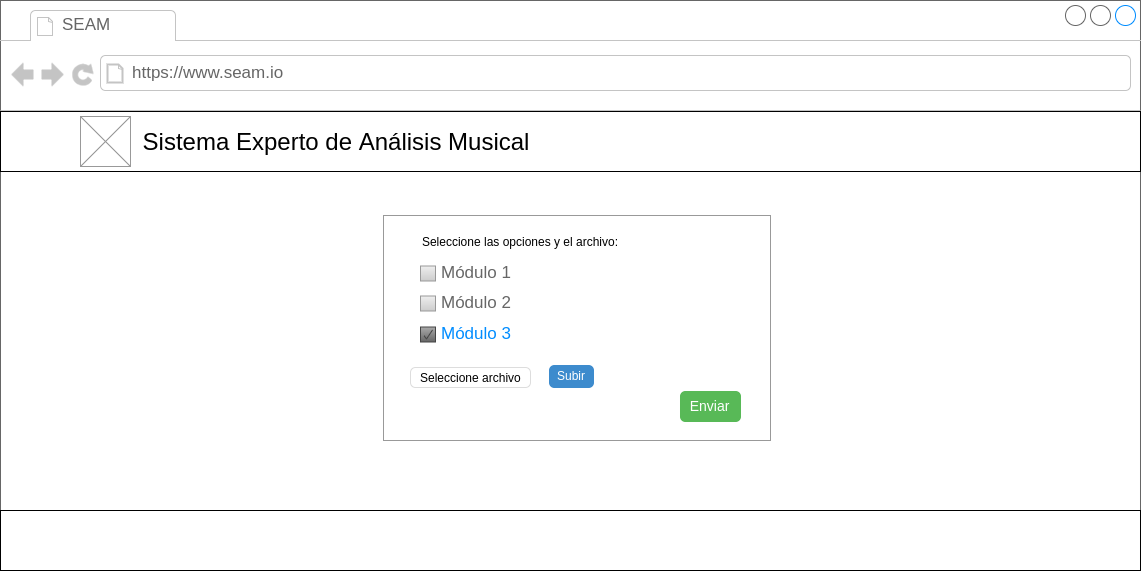
\includegraphics[scale=0.4]{imagenes/interfaz1.png}
	\caption{Wireframe de la página principal de la interfaz}
	\label{fig4.1.2.1}
\end{figure}

\begin{figure}[H]
	\centering
	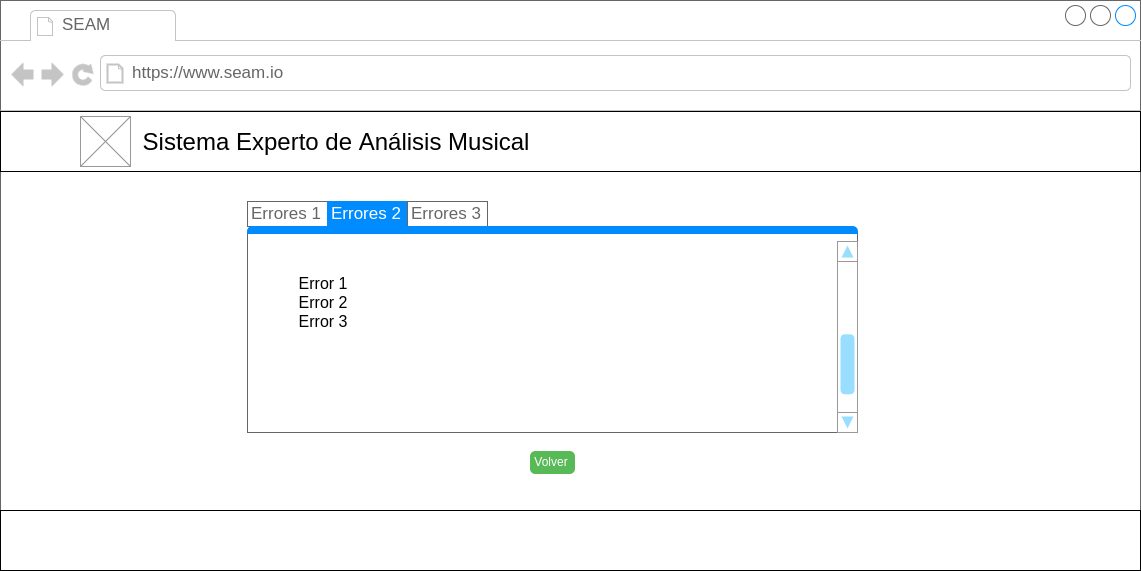
\includegraphics[scale=0.4]{imagenes/interfaz2.png}
	\caption{Wireframe de la página de resultados de la interfaz}
	\label{fig4.1.2.2}
\end{figure}

\bigskip
La paleta de colores utilizada se muestra en la figura \ref{fig4.1.2.3}.

\begin{figure}[H]
 	\centering
	
\includegraphics[scale=0.2]{imagenes/paleta.png}
	\caption{Paleta de colores de la interfaz}
	\label{fig4.1.2.3}
\end{figure}

El uso de cada color se describe a continuación:

\begin{itemize}
	
	\item El tono rojo se utilizará como fondo.
	\item Los tonos blanco y negro se utilizarán para el texto, y además el blanco para los fondos del formulario y la ventana de resultados.
	\item El tono gris claro se utilizará para resaltar algunos detalles.
	\item El tono gris oscuro se usará para la cabeza y el pie.
\end{itemize}

La maquetación de la interfaz se llevará a cabo haciendo uso de HTML5 y CSS3, apoyándonos en el sistema de temaplates Jinja2. Adicionalmente, se hará uso de jQuery para algunas funcionalidades.

\section{Arquitectura del sistema}

La arquitectura será \textbf{MVT} (Model-View-Template), que es la arquitectura empleada por DJango. En esta arquitectura, las vistas hacen el papel de ``controlador'' del sistema. Éstas serán las que contendrán al sistema experto.  

El sistema experto se dividirá en tres módulos:

\begin{itemize}

	\item Módulo 1: realizará la búsqueda de faltas en los acordes provocadas por los movimientos de las voces, como las faltas de quintas paralelas, octavas paralelas o duplicación de sensibles.

	\item Módulo 2: realizará el análisis melódico para señalar todos los errores en las líneas melódicas y su contrapunto.

	\item Módulo 3: comprobará la lógica tonal del coral y comprobará las secuencias de acordes, así como que estos se encuentren completos. 

\end{itemize}

En imagen \ref{fig4.2.1} se muestra gráficamente cómo sería la arquitectura del sistema.

\begin{figure}[H]
	\centering
	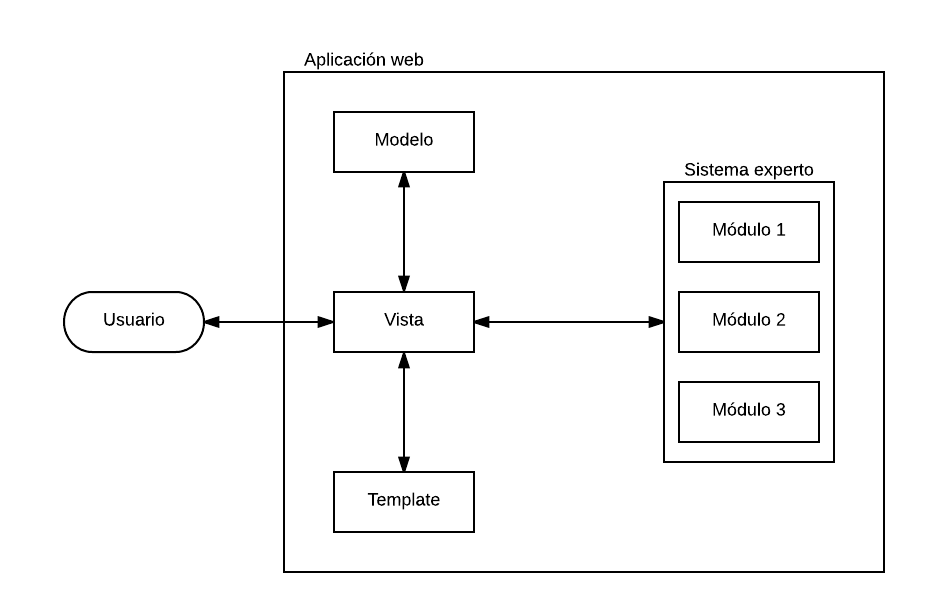
\includegraphics[scale=0.8]{imagenes/arquitectura.png}
	\caption{Diagrama de la arquitectura del sistema}
	\label{fig4.2.1}
\end{figure}
\chapter{Implementación}

La implementación de este proyecto se ha llevado a cabo en dos fases diferenciadas: la creación del sistema experto y el desarrollo de la aplicación web,utilizada como interfaz, en la que será embebido. 

Todo el código puede ser consultado en \cite{CODIGO}.

\section{Sistema experto}

El primer paso fue la creación de un prototipo utilizando el entorno de CLIPS. A continuación, se explican las decisiones tomadas a lo largo del desarrollo de este prototipo.

\subsection{Formato de los datos de entrada: partitura}

Una de las primeras cuestiones fue cómo obtener la información necesaria del XML en el que está contenida la partitura. Dado que CLIPS no puede procesar el XML para leer el contenido de las etiquetas, está funcionalidad tenía que ser realizada por Python. Sin embargo, definimos las estructuras que debían tener los ficheros para poder ser leídos por CLIPS y añadir esa información en forma de hechos.

Los datos que teníamos que extraer de la partitura eran:

\begin{itemize}

	\item La \textbf{tonalidad} de la obra. La tonalidad es la que nos define la \textit{escala musical} sobre la que está construido el coral. Nos da la relación entre los acordes y sus funciones tonales. La tonalidad está compuesta por el nombre y el modo.

	\item El \textbf{compás}. El compás nos indica cuántas figuras de un determinado tipo hay en cada pulso. El compás está compuesto por dos números que nos indican el número de pulsos y el tipo de figura que dura un pulso:

	\begin{itemize}
		\item 1: redonda
		\item 2: blanca
		\item 4: negra
		\item 8: corchea
	\end{itemize}

	\item Las \textbf{notas} de cada voz. Las notas musicales vienen definidas por su nombre, su altura, su duración y su alteración.

	\item Los \textbf{movimientos} de cada voz. Los movimientos nos indican si la voz, de una nota a otra, se mueve de forma ascendente, descendente o se mantiene.

\end{itemize}

Para cada uno de estos datos se creo una plantilla con la instrucción ``\texttt{deftemplate}'', al igual que para el resto de hechos como se mencionó en el capítulo \textit{Adquisición de conocimientos}. 

\subsubsection{Estructura del archivo de notas}

Una de las mayores dificultades fue decidir la estructura del archivo que contendría la información sobre las notas. Cada nota tiene una duración independiente, lo cual a la hora de realizar el análisis armónico resulta muy complejo. Al analizar la armonía de una obra tenemos que tener en cuenta todas las voces al mismo tiempo, analizamos de forma vertical. Sin embargo, en una misma parte cada nota de cada voz puede tener una duración distinta y por ende puede formarse más de un acorde en dicha parte. Esto significa que no siempre va a haber el mismo número de acordes, ni de notas, en cada compás.

En la práctica, a un experto este hecho no le resulta un problema, porque puede observar las voces gráficamente y poder determinar cuándo termina la duración de cada nota y el acorde. En cambio, para un sistema experto, al no saber dónde termina cada nota con respecto a las demás, no puede hacer esas deducciones de manera tan sencilla. 

Para solucionar este problema, decidí subdividir todas las notas de todas las voces a semicorcheas, que es la figura musical más pequeña que se suele utilizar en los corales. De esta forma, conseguimos que en todos los compases haya el mismo número de notas en cada voz.

En la siguiente figura, se muestra gráficamente lo que supone esta transformación:


\begin{figure}[H]
	\centering
	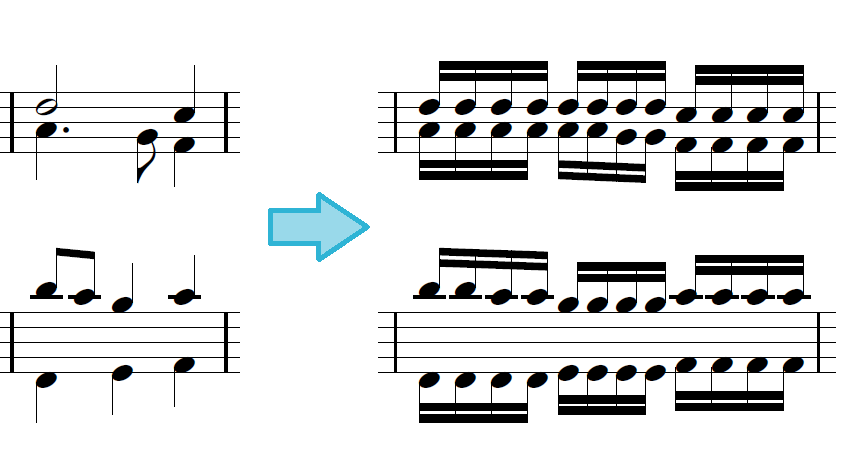
\includegraphics[scale=0.5]{imagenes/division.png}
	\caption{Subdivisión de un compás del coral ``Aus meines Herzens Grunde'' de \textit{J.S.Bach} a semicorcheas}
	\label{fig5.1.1}
\end{figure}

Como podemos ver, al realizar esta subdivisión podemos ir analizando en bloques equivalente en tiempo. Los resultados del análisis no se ven afectados, dado que únicamente hemos modificado la duración de las notas, la cual no interviene en los errores que vamos a detectar.

En el caso del análisis melódico, no es necesario hacer esta subdivisión porque analizamos cada voz de manera independientede de las otras, analizamos la partitura horizontalmente.

\subsubsection{Formatos finales}

Las estructuras de los ficheros que leería el sistema experto quedarían de la siguiente manera:

\begin{itemize}

	\item Fichero de la tonalidad:

		\begin{lstlisting}[frame=single]

			Nombre Modo

		\end{lstlisting}

		Ejemplo:

		\begin{lstlisting}[frame=single]

			D Mayor

		\end{lstlisting} 

	\bigskip
	\item Fichero del compás:

		\begin{lstlisting}[frame=single]

			Partes Figura

		\end{lstlisting}

		Ejemplo:

		\begin{lstlisting}[frame=single]

			3 4

		\end{lstlisting} 

	\bigskip
	\item Fichero de notas: se crearía un fichero para cada voz.
	
		\begin{lstlisting}[frame=single]

			Nombre Alteracion Altura Nombre Alteracion Altura ...

		\end{lstlisting} 

		Ejemplo:

		\begin{lstlisting}[frame=single]

			A b 4 B 2 D s 3

		\end{lstlisting} 

	\bigskip
	\item Movimientos:

		\begin{lstlisting}[frame=single]

			Movimiento1 Movimiento2 Movimiento3 ...

		\end{lstlisting} 

		Ejemplo:

		\begin{lstlisting}[frame=single]

			Ascendente Ascendente Descendente

		\end{lstlisting} 

\end{itemize}

Los nombres de las notas se representarán con el cifrado americano, el empleado en el archivo XML. La equivalencia entre el cifrado americano y el empleado en occidente es:

\begin{itemize}

	\item Do $\rightarrow$ C
	\item Re $\rightarrow$ D
	\item Mi $\rightarrow$ E
	\item Fa $\rightarrow$ F
	\item Sol $\rightarrow$ G
	\item La $\rightarrow$ A
	\item Si $\rightarrow$ B

\end{itemize}

\subsection{Implementación del primer prototipo}

En el primer prototipo, no se modularizaron los hechos y reglas en función de los módulos descritos en los capítulos anteriores. Esto es porque aún no estaban definidas del todo las dependencias de las reglas respecto a los hechos ni la división del análisis armónico en dos partes realmente diferenciadas. 

Aunque en el análisis y el diseño quedan claras estas divisiones, a la hora de implementar las reglas, iban surgiendo muchas relaciones entre todos los hechos de la base de conocimiento. Por ejemplo, se esperaba que los hechos referidos a los movimientos de las voces únicamente fueran utilizados por el módulo del análisis melódico. Sin embargo, también es necesario para localizar algunos errores armónicos. Además, la existencia de algunos errores melódicos provoca a su vez errores armónicos y viceversa. 

Una vez se terminaron de implementar todas las reglas y hechos, se procedió a verificar y validar el prototipo. 

La  \textbf{verificación} consistió en comprobar que los ficheros se leían correctamente y los hechos deducidos se asertaban en el sistema de la manera esperada. Esto se comprobó fácilmente observando la ventana de hechos que aparece en la propia interfaz de CLIPS.

La \textbf{validación} se realizó creando archivos de prueba, con los formatos descritos anteriormente, que contuviesen al menos un error de cada tipo. Los modelos de prueba fueron recogidos de las fuentes bibliográficas, las cuáles contienen una gran cantidad de ejemplos

\subsection{Modularización del sistema}

Tras la creación del primer prototipo y su verificación y validación, comencé el proceso de modularización del sistema. 

Al estar implementadas todas las reglas y funcionalidades del sistema, este proceso, aunque tedioso, fue el más sencillo. 

Fui comprobando para cada regla los antencendentes que debían cumplirse y así poder agruparlas según los hechos que necesitaban.
Una vez agrupadas, pude definir los hechos asertados necesarios para cada uno de los módulos.

Como resultado final, obtuve los tres módulos de análisis, cada uno con sus reglas y hechos diferenciados. 

\section{Aplicación web}

La implementación de la aplicación web, como se comentó en el capítulo anterior, se ha hecho utilizando el framework DJango de Python.

La finalidad de implementar esta aplicación es proporcionar al sistema experto una interfaz agradable y sencilla de utilizar para el usuario. 

Este portal se encargará de las siguientes funciones:
\begin{itemize} 
	\item El envío de un formulario con las opciones de análisis seleccionadas por el usuario y el archivo de la partitura a analizar.
	\item La extracción de datos del archivo XML de la partitura y escritura de los mismos en ficheros según se describe en la sección anterior.
	\item La ejecución de los módulos seleccionados del sistema experto.
	\item Mostrar los errores detectados.
\end{itemize}

\subsection{Tratamiento del archivo XML}

Como se ha comentado antes, CLIPS no puede extraer la información de las etiquetas del archivo XML. Esta tarea es implementada por Python haciendo uso de la API \textit{ElementTree XML}. Esta API nos permite buscar etiquetas y leer el contenido de las mismas. 

Los archivos XML que contienen partituras, hacen uso de una gran cantidad de etiquetas. En este caso, para extraer los datos necesarios consultamos las siguientes:

\begin{itemize}

	\item \textit{Key}: para extraer la tonalidad.
	\item \textit{Time}: para extraer el compás.
	\item \textit{Note}: para extraer información de la nota. Dentro de ésta consultamos la siguientes subetiquetas:
		\begin{itemize}
			\item \textit{Pitch}: para extraer el nombre y la octava. 
			\item \textit{Accidental}: para comprobar si tenía una alteración accidental.
			\item \textit{Type} y \textit{Dot}: para extraer la duración.
			\item \textit{Voice}: para extraer la voz que canta dicha nota.
		\end{itemize}
\end{itemize}

La información contenida en las etiquetas se escribe en ficheros de acuerdo al formato que definimos.

\subsubsection{Determinación de movimientos melódicos}

Para el análisis melódico y algunas cuestiones del análisis armónico es necesario conocer la dirección que van tomando las melodías. Esta información no viene representada de forma explícita en el archivo de la partitura, sino que debemos de extraerla nosotros. 

Una vez se han creado los archivos que contienen las notas de las voces, vamos comprobando las notas dos a dos para determinar si la melodía hace un movimiento descendente, ascendente o se mantiene. 

La lista de movimientos de cada voz se escribe en un fichero para ser utilizado por los módulos de análisis.

\subsection{Integración del sistema experto}

Esta fase de la implementación fue la que presentó más problemas. Para integrar el sistema con la interfaz web he utilizado la librería PyCLIPS. Esta librería permite utilizar las funciones de CLIPS para crear sistema expertos en Python. Además, también permite cargar archivos creados en CLIPS y ejecutarlos.

Gracias a esta última característica, en un principio se pensó que únicamente sería necesario cargar los archivos de los módulos y  ejecutarlos cuando fuera necesario. Sin embargo, hubo que hacer algunas modificaciones.

El primer problema con el que me encontré fue que los archivos no podían cargarse. Tras buscar en la documentación de PyCLIPS \cite{PYCLIPS}, encontré la respuesta a este problema. PyCLIPS permite cargar archivos de CLIPS que contengan reglas o hechos, pero no ambas en un mismo fichero. Así pues, dividí los ficheros en ficheros con reglas y ficheros con hechos. 

De nuevo, surgió otro problema, esta vez con los archivos de hechos. En este caso, no se aceptaban las definiciones de las estructuras \texttt{deftemplate}. Para solucionarlo, decidí añadirlas utilizando explícitamente las funciones de PyCLIPS. A pesar de que parecía haberse solucionado, esto derivó en nuevos problemas asociados a dos funciones de CLIPS: las funciones \texttt{clear} y \texttt{reset}.

\bigskip
La función \texttt{clear} borra todo el entorno de CLIPS, eliminando de la memoria de trabajo todos los hechos, reglas, plantillas y funciones que estuviesen definidos.

\bigskip
La función \texttt{reset} reinicia el entorno, eliminando sólo los hechos y dejando en la memoria de trabajo todas las reglas, plantillas y funciones.

\bigskip

Antes de la ejecución de cada módulo se siguen los siguientes pasos:

\begin{itemize}
	\item Se transforma el XML a los archivos de entrada del sistema experto.
	\item Se limpia el entorno.
	\item Se reinicia el entorno.
	\item Se cargan las plantillas del módulo.
	\item Se cargan los hechos del módulo.
	\item Se cargan las reglas del módulo.
\end{itemize}

Debido a algún problema con la librería PyCLIPS o el intérprete de Python, la función \texttt{clear} no puede ejecutarse. Esto provoca que cada vez que se lancen los módulos del sistema, se redefinan las plantillas con las funciones de PyCLIPS. CLIPS no permite sobreescribir hechos o plantillas, por lo que nos daba un error de redefinición. 

Para el correcto funcionamiento del sistema, las plantillas debían ser definidas una única vez al inicio del sistema. Tras consultar la documentación y el foro de la comunidad encontré la solución: había que definir las plantillas en el archivo \texttt{urls.py}. Este archivo contiene las expresiones regulares de las ``urls'' en las que se visualizarán las secciones de la pagina web. Éste código se ejecuta una única vez al inicio de la aplicación, lo que nos permite evitar que las plantillas se creen una y otra vez.

Aunque se solucionó el problema de las plantillas, no se podía leer el archivo de hechos. Para asertar conjuntos de hechos en el entorno de CLIPS se utiliza la instrucción \texttt{deffacts}. Esta instrucción no era reconocida por la función \texttt{LoadFacts} de PyCLIPS, que es la encargada de cargar el archivo. Intenté modificar la sintaxis del archivo utilizando otras instrucciones como \texttt{assert}, que ``aserta'' los hechos en la memoria de trabajo, o escribiendo directamente los hechos, sin éxito. Al igual que con la función \texttt{clear}, no conseguía hacer que la función \texttt{LoadFacts} se ejecutase correctamente. 

Finalmente, opté por almacenar el contenido de los hechos en archivos independientes - un archivo por tipo de \texttt{template} - y añadir nuevas reglas para la lectura de estos ficheros y la creación de los hechos correspondientes. 

\bigskip
Algunos de estos problemas referidos a funciones e instrucciones que no se ejecutan o dan errores de ejecución se deben principalmente a que PyCLIPS define los hechos, reglas y demás elementos de CLIPS como objetos. Esto hace que se den problemas de asignación y liberación de memoria, como en el caso de la instrucción \texttt{clear}, entre otros. 

También comprobé que el uso de PyCLIPS mediante comandos en la consola no daba ninguno de estos problemas. Esto sugiere que quizá haya algún problema con el intérprete a la hora de ejecutar scripts que contengan código de esta librería.

\bigskip
En cualquier caso, una vez se solucionaron estos problemas, se pudo completar la integración del sistema de manera satisfactoria.

\subsection{Visualización de errores}

Se contemplaron varias posibilidades para mostrar los errores:

\begin{itemize}
	\item Mostrar los errores en tiempo real según fuesen encontrados por el sistema.
	\item Mostrar las listas completas de errores tras finalizar todo el proceso de análisis.
	\item Mostrar gráficamente la sección de la partitura en la que se detecte un error, señalizando de alguna manera las notas implicadas.
\end{itemize}

\bigskip
\bigskip

De estas opciones, se decidió que la segunda cumplía mejor con los requisitos de los usuarios. Esto se debe al hecho de que los errores que detecta el sistema, aunque se encuentren localizados en un compás concreto de la partitura, el ámbito al que afecta el error no es local sino global. Esto quiere decir que un error puede afectar al resto de la partitura al ser corregido generando nuevos errores, agravando otros o incluso solucionando otros problemas posteriores. 

Por este motivo, mostrar los errores en tiempo real no le resulta tan útil al usuario como mostrar la lista completa. El tener la lista completa permite tener una visión general de todas las faltas y errores. 

De igual manera, el hecho de mostrarlo gráficamente no resultaba especialmente útil por la posibilidad de que existan secciones que se repitan o se parezcan a lo largo de la obra, dificultando la señalización concreta de los errores. 

En todos los errores encontrados se especifica el compás, la parte, el tipo de error encontrado, las voces involucradas y una explicación sobre el mismo, haciendo alusión al porqué es producido y la razón por la que no debe darse. Si no se encontrasen errores, el sistema mostraría un mensaje de éxito.

\section{Aspecto final}

En las siguientes figuras podemos ver cuál ha sido el aspecto final de este sistema:

\bigskip

\begin{figure}[H]
	\centering
	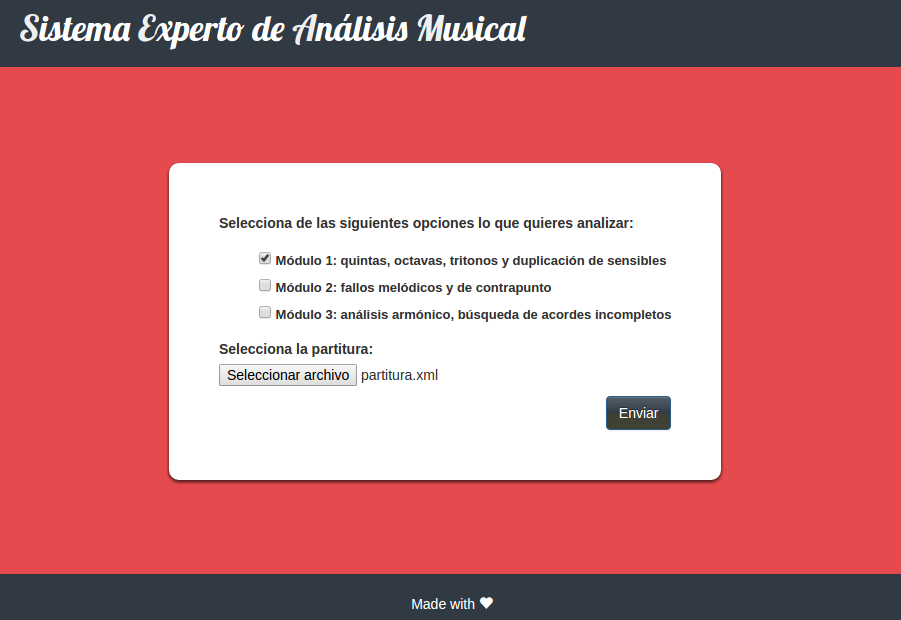
\includegraphics[scale=0.35]{imagenes/interfaz3.png}
	\caption{Página principal}
	\label{fig5.3.1}
\end{figure}

\begin{figure}[H]
	\centering
	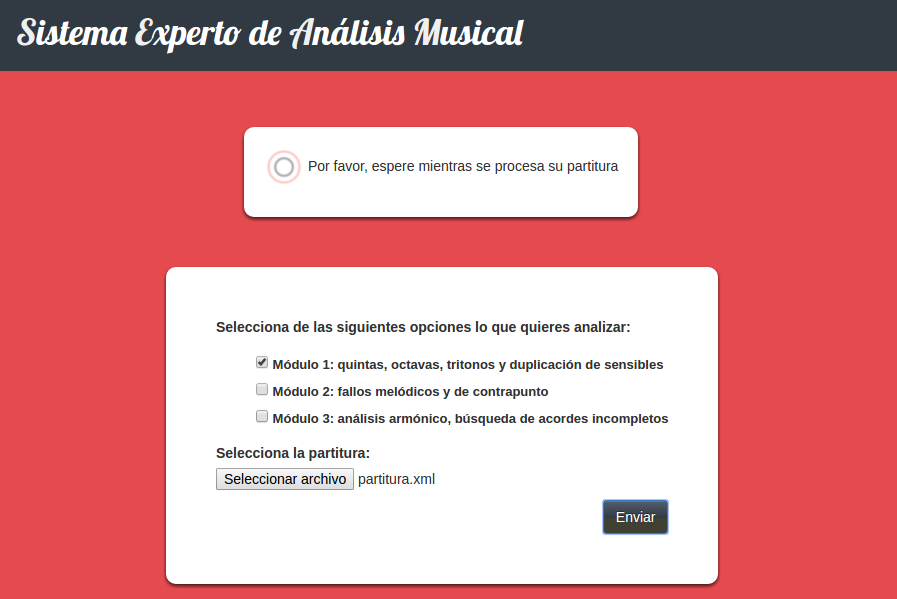
\includegraphics[scale=0.35]{imagenes/interfaz4.png}
	\caption{Página principal tras enviar el formulario}
	\label{fig5.3.2}
\end{figure}

\bigskip

\begin{figure}[H]
	\centering
	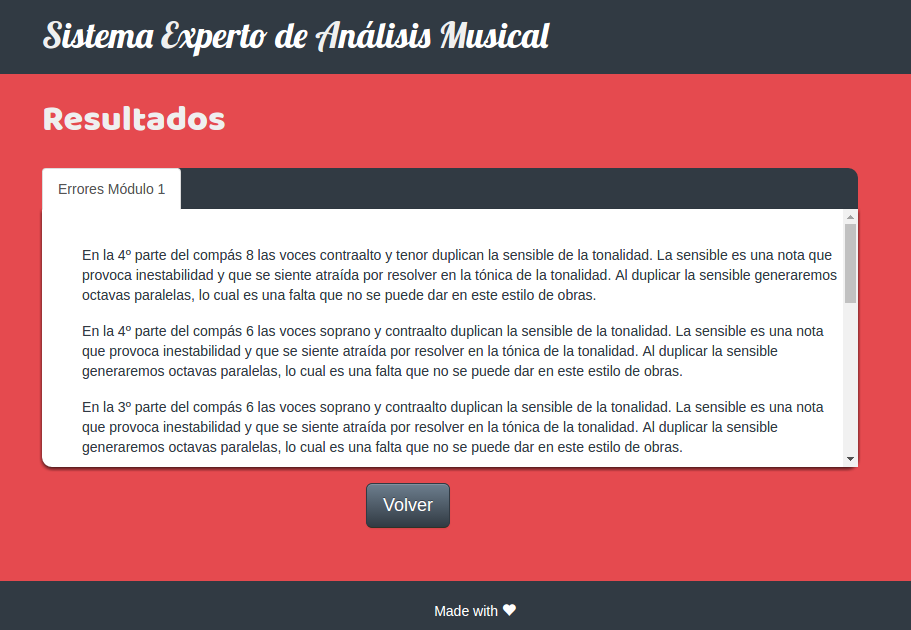
\includegraphics[scale=0.35]{imagenes/interfaz5.png}
	\caption{Visualización de resultados con errores}
	\label{fig5.3.3}
\end{figure}

\begin{figure}[H]
	\centering
	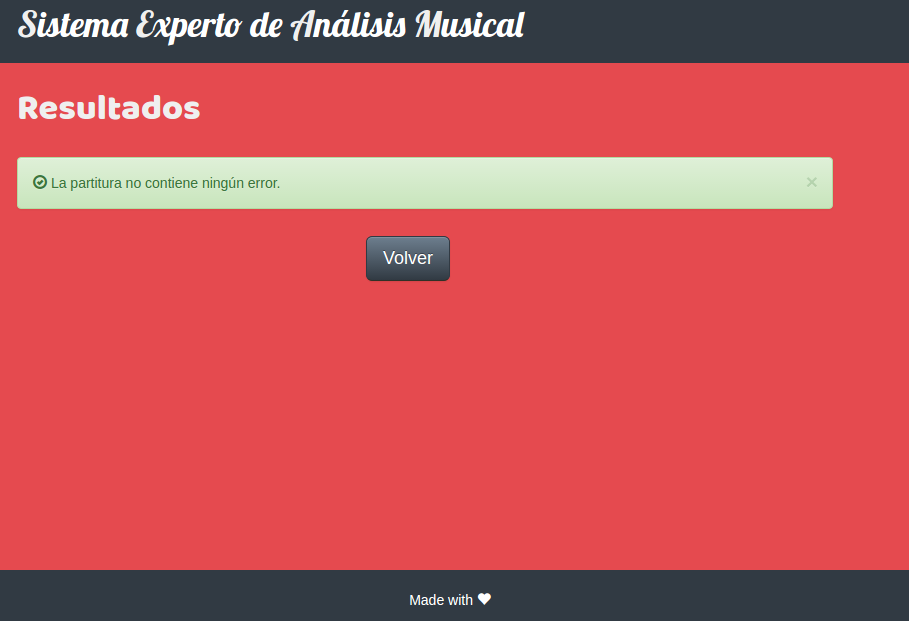
\includegraphics[scale=0.35]{imagenes/interfaz6.png}
	\caption{Visualización de resultados sin errores}
	\label{fig5.3.4}
\end{figure}
\chapter{Pruebas y validación}

Con toda la implementación del sistema realizada, pasamos a la fase de verificación y validación del sistema. 

\section{Verificación}

Como describimos en el capítulo anterior, la verificación del sistema experto consistió en comprobar que accedía y leía bien el contenido de los ficheros y añadía los hechos a la memoria de trabajo de manera correcta. 

Como no podíamos comprobarlo visualmente como hicimos con el prototipo, se hicieron pruebas en las que el sistema experto, además de los errores, mostraba los hechos asertados, hechos calculados y hechos leídos. 

Una vez se comprobó que el sistema experto se ejecutaba correctamente, pasamos a comprobar las funcionalidades de la interfaz.

Primero se comprobó que las funciones de extracción de información del archivo XML obtenían y guardaban correctamente los datos. Para ello, se ejecutaron todas las funciones con distintas partituras y se revisaron los ficheros resultantes para ver si coincidían con el formato escogido y no contenían fallos.

También se verificó el funcionamiento del envío del formulario para que no se produjesen las siguientes situaciones:

\begin{itemize}

	\item No se puede enviar un formulario en blanco.
	\item No se puede enviar un archivo sin seleccionar ninguna opción.
	\item No se puede enviar la lista de opciones sin adjuntar un archivo.
	\item El archivo a adjuntar debe ser de formato XML.

\end{itemize}

Por último, se examinó que los resultados se mostrasen de manera legible y ordenados en sus pestañas correspondientes. Las pestañas de los módulos deben mostrarse si se ha seleccionado dicho módulo y si se han obtenido errores. En caso contrario, no deberían de mostrarse.

\section{Validación}

La validación del sistema experto fue llevada a cabo por Clara Luz Fernández Vecino, profesora de armonía del Conservatorio Ángel Barrios de Granada.

Para ello, el sistema analizó ejercicios realizados por los alumnos del conservatorio:

\begin{itemize}

	\item Alrededor de 100 ejercicios de armonía. Con estos ejercicios se validaron los módulos de errores provocados por los movimientos y algunos errores armónicos. 

	\item 20 ejercicios de composición de corales. Con estas composiciones se validaron todos los módulos, especialmente el módulo de análisis melódico.

\end{itemize}

Tras ejecutar el sistema, Clara Luz revisó los resultados obtenidos por el sistema comparándolos con las correcciones que ella misma había llevado a cabo sobre todos los ejercicios.
\chapter{Resultados y conclusiones}

\section{Resultados}

Los resultados obtenidos tras la validación del sistema por Clara Luz han sido entre un 85-90\% de acierto. Esto significa que de todos los errores señalados por Clara Luz, el sistema detecto el 85-90\% de todos ellos aproximadamente.

En los casos de errores no detectados, se debía a que eran situaciones extremas o excepcionales que no había considerado para el desarrollo del sistema, como por ejemplo resoluciones excepcionales de séptimas o detección de quintas paralelas entre acordes sin tener en cuenta las notas de paso. 

Sin embargo, el sistema en muchos de los ejemplos, fue capaz de detectar errores que no habían sido encontrados por Clara Luz. Esta cantidad de errores podían ser desde encontrar un error no señalizado a incluso diez o más, por lo que es difícil estimar un porcentaje claro.

Si no tenemos en cuenta el porcentaje de error debido a casos no contemplados por el sistema o no implementados, el sistema encuentra prácticamente todos los errores, suponiendo un 95\% o más de acierto.

\bigskip

Respecto al tiempo empleado para analizar las partituras, si comparamos el tiempo empleado por el sistema con la interfaz web y sin ella, los resultados no son muy favorables. La ejecución del sistema experto en el entorno de CLIPS tarda unos pocos segundos, mientras que con la interfaz tarda entre 1 y 5 minutos. 

\section{Conclusiones}

En relación a los resultados referidos al porcentaje de errores encontrados, considero que dada la complejidad de la tarea, se han obtenido buenos resultados. 

He de destacar el hecho de que el sistema encontró errores que no habían sido señalados por Clara Luz. Esto supone que el sistema, en algunas ocasiones, puede analizar partituras mejor o con más detalle que un experto. Obviamente en el caso del experto siempre está el factor humano y la garantía de cometer errores más fácilmente que una máquina. Aún así, este hecho fue una muy grata sorpresa.

También destacar el hecho de que si en la partitura se encuentra alguno de los errores o faltas que se describen en los requisitos, siempre es capaz de detectarlos y señalarlos, lo cual satisface por completo los objetivos propuestos.

\bigskip
En cuanto a los resultados sobre el tiempo de ejecución, el hecho de crear la interfaz web ha supuesto una pérdida de velocidad considerable. 

Al haber embebido el sistema dentro de una aplicación web, se ha perdido una de las mejores características de CLIPS, que es su velocidad de procesamiento. Esta ventaja de CLIPS se ha sacrificado para poder hacer un sistema más accesible y con una interfaz más afable, dado que es muy improbable que los usuarios finales tengan algún conocimiento sobre CLIPS o su existencia. 

Por otro lado, para un experto, estos análisis tan exhaustivos pueden llevar alrededor de 20 minutos para un coral de 24-32 compases, que suele ser la longitud media de este tipo de obras. Teniendo en cuenta esta comparación, el sistema tarda, como mínimo, cuatro veces menos que un experto, lo cual supone una ganancia en tiempo bastante aceptable.

Dado que el tiempo no era realmente un requisito indispensable o un objetivo propuesto no le he dado demasiada importancia a la pérdida de eficiencia que nos ha supuesto la interfaz, y más si tenemos en cuenta que para el usuario supone una mejora respecto a hacer el análisis manualmente. 

Aún así he realizado algunas pruebas y mediciones sobre la ejecución del sistema con la interfaz. He podido comprobar que la pérdida de velocidad no radica en la ejecución del sistema experto sino que parece estar más bien relacionada con procesar los resultados para poder mostrarlos de manera correcta. Esto significa que el problema no está relacionado con la implementación del sistema experto sino con alguno de los procedimientos que se llevan a cabo en la interfaz o con su conexión entre el servidor y el usuario.

\bigskip

Teniendo en cuenta todo lo anterior, podemos concluir que este sistema proporciona unos resultados bastante buenos en un tiempo bastante aceptable y que hemos podido satisfacer todos los requisitos y alcanzar los objetivos propuestos.

\section{Futuro desarrollo}

Uno de los motivos principales por los que se escogió hacer un sistema experto es por su gran escalabilidad. Este proyecto puede ser ampliado en una gran cantidad formas:

\begin{itemize}

	\item Añadiendo nuevas reglas de armonía y/o excepciones a los módulos de análisis ya existentes.
	\item Añadiendo nuevos módulos para analizar otros aspectos o estilos musicales.
	\item Adaptando los módulos a otros tipos de obras y formas musicales, como obras para piano, orquesta, ...
	\item Añadir nuevas funcionalidades a la aplicación como creación de usuarios, llevar un registro de las partituras analizadas, añadir estadísticas, ...
\end{itemize}

\bigskip

Además, está el hecho de que se puede intentar mejorar la eficiencia del sistema utilizando programación concurrente, mejorando el uso de la memoria o incluso intentar trasladarlo a otro tipo de interfaz que pueda ser más eficiente en términos de velocidad.

\bigskip
En definitiva, este sistema aún tiene muchas posibilidades de mejorar y crecer, aunque como primera versión ha dado unos resultados más que satisfactorios.

%----------------------------------------------------------------------------------------
%	Glosario
%----------------------------------------------------------------------------------------
\chapter*{Anexo: Glosario}
\addcontentsline{toc}{chapter}{Anexo: Glosario}
\label{glosario}


\begin{itemize}[label={}, leftmargin=*]
	
	\label{acorde}
	\item \textbf{Acorde}: conjunto de tres o más notas diferentes que suenan simultáneamente y que constituyen una unidad armónica. Las notas que forman los acordes de triada o tres notas se denominan: \textit{fundamental} - nota sobre la que se construye el acorde -,  \textit{tercera} - nota que forma un intervalo de tercera con la fundamental - y \textit{quinta} - nota que forma un intervalo de quinta con la fudamental. En el caso de acordes de cuatriada o cuatro notas, además de las notas que se mencionan, aparece la \textit{séptima} - nota que forma un intervalo de séptima con la fundamental.

	\begin{itemize}

			\label{inversion}
			\item \textbf{Acorde invertido}: se dice que un acorde está \textit{invertido} cuando la nota más grave no es la fundamental, sino alguna de las otras que forma el acorde. Si se forma sobre la tercera, el acorde está en \textit{primera inversión}; si se construye sobre la quinta, está en \textit{segunda inversión} y si se construye sobre la séptima, está en \textit{tercera inversión}.

	\end{itemize}

	\bigskip

	\label{alteracion}
	\item \textbf{Alteraciones}: signos que modifican la entonación o altura de los sonidos naturales y alterados. Las alteraciones más utilizadas son el \textit{sostenido} \sharp{} , el \textit{bemol} \flat{} y el \textit{becuadro} \natural{}. 

	\begin{itemize}

		\item \textbf{Alteraciones propias}: aquellas que se colocan al principio del pentagrama. Éstas son determinadas por la \textit{tonalidad} de la obra. También se les llama \textit{armadura}.

		\label{accidental}
		\item \textbf{Alteraciones accidentales}: aquellas que aparecen en cualquier punto de la partitura, modificando temporalmente a la nota que acompañan.

	\end{itemize}

	\bigskip

	\label{armonico}
	\item \textbf{Análisis armónico}: estudio, a partir de la tonalidad de la obra, de los \textit{acordes}, \textit{grados}, \textit{inversiones} y \textit{funciones} que componen a la misma y las relaciones entre ellos.

	\bigskip

	\label{melodico}
	\item \textbf{Análisis melódico}: estudio de la melodía o línea melódica para determinar si está bien construida, es decir, si es fluida y consistente con la \textit{armonía} sobre la que se basa.

	\bigskip

	\label{armadura}
	\item \textbf{Armadura}: conjunto de \textit{alteraciones} propias de una tonalidad escritas al principio de un pentagrama, entre la \textit{clave} y el \textit{compás}. Determina qué notas deben ser interpretadas de manera sistemática un semitono por encima o por debajo de sus notas naturales (no alteraradas) equivalentes.

	\bigskip

	\label{armonia}
	\item \textbf{Armonía}: disciplina de la música en la que se estudian los acordes y sus relaciones para producir sensaciones sonoras, sensaciones de relajación o sosiego (consonancia)  y de tensión (disonancia). 

	\begin{itemize}

		\item \textbf{Armonía clásica} o \textbf{armonía tradicional}: referida a la armonía tonal o funcional. La armonía tonal es la empleada desde la época Prebarroca (siglo XV) hasta el Romanticisimo (siglo XIX). 

	\end{itemize}

	\bigskip

	\label{coherencia}
	\item \textbf{Coherencia musical}: decimos que una obra o melodía es coherente cuando ésta tiene fluidez y es consistente.

	\bigskip

	\label{conduccion}
	\item \textbf{Conducción melódica}: referida a la dirección y \textit{movimientos} entre las notas de una melodía. 

	\bigskip

	\label{consonancia}
	\item \textbf{Consonancia}: percepción subjetiva según la cual se consideran ciertos \textit{intervalos} musicales menos tensos que otros. Conjunto de sonidos que el oído percibe de forma distendida, agradable.

	\bigskip

	\label{contrapunto}
	\item \textbf{Contrapunto}: técnica de composición musical que evalúa la relación existente entre dos o más voces independientes  con la finalidad de obtener cierto equilibrio armónico.

	\bigskip

	\label{compás}
	\item \textbf{Compás}: entidad métrica musical compuesta por varias unidades de tiempo (\textit{figuras musicales}) que se organizan en grupos. Se especifica cuántos \textit{pulsos} o partes hay en cada compás y qué figura musical define un pulso.

	\bigskip

	\label{coral}
	\item \textbf{Coral}: obra para canto al unísono (una sola melodía) o polifónico (varias melodías).

	\bigskip

	\label{disonancia}
	\item \textbf{Disonancia}: percepción subjetiva según la cual se consideran ciertos \textit{intervalos} musicales más tensos que otros. Conjunto de sonidos que el oído percibe de forma desagradable o tiende a rechazar.

	\bigskip

	\label{escala}
	\item \textbf{Escala}: conjunto de sonidos ordenados, notas de un entorno sonoro particular, de manera simple y esquemática. Estos sonidos puede estar dispuestos de forma ascendente (de grave a agudo) o de forma descendente (de agudo a grave), uno a uno en posiciones específicas dentro de la escala, llamadas \textit{grados}.

	\bigskip

	\label{estructura}
	\item \textbf{Estructura armónica}: referido al conjunto de \textit{acordes} que conforman una obra. 

	\bigskip

	\label{figura}
	\item \textbf{Figura musical}: signo que representa gráficamente la duración de una nota. Las figuras más conocidas son la redonda \wholeNote{}, blanca \halfNote{}, negra \quarterNote{}, corchea \eighthNote{}, semicorchea \sixteenthNote{} y fusa \thirtysecondNote{}.

	\bigskip

	\label{forma}
	\item \textbf{Forma musical}: referida a la estructura de la obra o tipo. Ejemplos: coral, sonata, sinfonía, canción, ...

	\bigskip

	\label{funcion}
	\item \textbf{Función tonal} o \textbf{función armónica}: referida al grado de reposo o de inestabilidad (tensión) que aportan los \textit{grados} de una tonalidad. Las funciones tonales son \textit{tónica} (pasajes en reposo), \textit{subdominante} (pasajes intermedios entre reposo e inestabilidad)  y \textit{dominante} (pasajes inestables). 

	\bigskip

	\label{grado}
	\item \textbf{Grado tonal}: referido a la posición de cada nota dentro de una \textit{escala}. Se designan mediante números romanos correlativos I, II, III, IV, V, VI y VII. Cada grado tiene asociada una \textit{función tonal}:

	\begin{itemize}

		\item[--] I: función de \textit{tónica}.
		\item[--] II: función de \textit{subdominante}.
		\item[--] III: función de \textit{tónica}.
		\item[--] IV: función de \textit{subdominante}.
		\item[--] V: función de \textit{dominante}.
		\item[--] VI: función de \textit{tónica}.
		\item[--] VII: función de \textit{dominante}.

	\end{itemize}

	\bigskip

	\label{intervalo}
	\item \textbf{Intervalo}: diferencia de altura entre dos notas, medida cuantitativamente (número) en \textit{grados} o notas naturales y cualitativamente (especie) en tonos y semitonos. Cuantitativamente pueden ser segundas, terceras, cuartas, quintas, sextas, séptimas u octavas. Cualitativamente puede ser mayores, menores, justos, aumentados o disminuidos.

	\bigskip

	\label{movimientos}
	\item \textbf{Movimientos}: referido a los movimientos que pueden darse entre dos notas. Los movimientos pueden ser a nivel melódico o armónico.

	\begin{itemize}

		\item \textbf{Movimientos melódicos}: movimientos que se produce al pasar de una nota a otra en una melodía. Puede ser un movimiento por grado conjunto - nos movemos a la nota continua ascendente o descendente - o un movimiento por salto - nos movemos a una nota no continua.

		\item \textbf{Movimientos armónicos}: movimientos que se producen en las notas -dos a dos- al pasar de un acorde a otro. Pueden ser movimientos \textit{directos} (ambas notas se mueven en la misma dirección) , movimientos \textit{paralelos} ( ambas notas se mueven en la misma dirección y manteniendo el mismo intervalo entre ellas) , movimientos \textit{contrarios} (ambas notas se mueven en direcciones contrarias) y movimientos \textit{oblicuos} (una nota se mantiene estática y la otra se mueve ascendente o descendentemente).

	\end{itemize}

	\label{pulso}
	\item \textbf{Pulso}: unidad básica que se emplea para medir el tiempo.

	\bigskip

	\label{sensible}
	\item \textbf{Sensible}: referida a la séptima nota de la escala que se encuentra a un semitono de la tónica de la tonalidad. También puede hacer referencia al VII grado de la escala, al acorde que se forma sobre dicho grado o a la función tonal que desempeña (dominante). 

	\bigskip

	\label{septima}
	\item \textbf{Séptima de dominante}: referida a la séptima del acorde que se forma sobre el acorde de \textit{dominante} de la \textit{tónica}.

	\bigskip

	\label{tonalidad}
	\item \textbf{Tonalidad}: conjunto de sonidos que están en íntima relación entre sí con respecto a un centro tonal o \textit{tónica}.

	\bigskip

	\label{tonica}
	\item \textbf{Tónica}: primer \textit{grado} de la \textit{escala} musical y es la nota que define la \textit{tonalidad}. 

\end{itemize}

%----------------------------------------------------------------------------------------
%	Referencias
%----------------------------------------------------------------------------------------
\newpage
\thispagestyle{empty}
\
\nocite{*}
\cleardoublepage
\phantomsection
\addcontentsline{toc}{chapter}{Bibliografía}
\bibliography{bibliografia} %archivo bibliografia.bib que contiene las entradas 
\bibliographystyle{apalike} 

\end{document}